\documentclass[11pt]{article}
\usepackage[margin=1.05in]{geometry}
\usepackage{graphicx}
\usepackage{booktabs}
\usepackage{xcolor}
\usepackage{microtype}
\usepackage{enumitem}
\usepackage{amsmath}
\usepackage[hidelinks]{hyperref}
\usepackage{caption}
\usepackage{tikz}
\captionsetup{font=small,labelfont=bf}
% Advanced AI Society brand palette (shared with the Society's other papers)
\definecolor{aailime}{HTML}{CFFF04}
\definecolor{aailimetint}{HTML}{F2FFB8}
\definecolor{aaiink}{HTML}{0A0A0A}
\definecolor{aaineutral}{HTML}{E7E3DD}
\definecolor{aaipaper}{HTML}{F0EDEA}
\definecolor{aaimuted}{HTML}{8F8A82}
\definecolor{aaidarklime}{HTML}{7A9900}
\colorlet{ink}{aaiink}
\colorlet{teal}{aaidarklime}
\colorlet{violet}{aaiink}
\setlist{nosep}
\renewcommand{\topfraction}{0.92}\renewcommand{\bottomfraction}{0.6}\renewcommand{\textfraction}{0.06}\renewcommand{\floatpagefraction}{0.75}
\setcounter{topnumber}{3}\setcounter{totalnumber}{4}
\newcommand{\vsla}{\textsc{vsla}}
\newcommand{\slsa}{\textsc{slsa}}
\newcommand{\lvl}[1]{\textbf{L#1}}

\title{\vsla: Supply-chain Levels for\\Machine-to-Machine Vulnerability Disclosure}
\author{Jim Schwoebel\\Quome, Inc.\ and Advanced AI Society\\\texttt{jim@quome.com}}
\date{October 30, 2026 \quad\textit{draft v1.0}}

% ------------------------------------------------------------------ cover page
\newcommand{\glance}[3]{%
  \begin{tikzpicture}[baseline=(current bounding box.north)]
    \node[draw=#1, line width=0.9pt, rounded corners=9pt, fill=#1!5, inner xsep=10pt, inner ysep=9pt, text width=0.275\textwidth, minimum height=2.6cm, align=left, anchor=north west]
      {{\scriptsize\sffamily\bfseries\color{#1}\MakeUppercase{#2}}\\[0.3em]{\footnotesize #3}};
  \end{tikzpicture}}

% The Society's bracket mark, drawn natively (lime on the dark band)
\newcommand{\aaimark}[1]{%
\begin{tikzpicture}[x=#1, y=#1, line cap=butt]
  \fill[aailime] (0,0) rectangle (0.16,1);
  \fill[aailime] (0.16,0) rectangle (0.42,0.24);
  \fill[aailime] (0.16,0.76) rectangle (0.42,1);
  \fill[aailime] (1.04,0) rectangle (1.20,1);
  \fill[aailime] (0.78,0) rectangle (1.04,0.24);
  \fill[aailime] (0.78,0.76) rectangle (1.04,1);
\end{tikzpicture}}

\begin{document}
\thispagestyle{empty}

\begin{tikzpicture}[remember picture, overlay]
  \fill[aaiink] (current page.north west) rectangle
    ([yshift=-6.35cm]current page.north east);
  \fill[aailime] ([yshift=-6.35cm]current page.north west) rectangle
    ([yshift=-6.53cm]current page.north east);
  \node[anchor=north west, inner sep=0pt]
    at ([xshift=1.05in, yshift=-0.95cm]current page.north west) {\aaimark{0.62cm}};
  \node[anchor=north west, inner sep=0pt, text width=14.2cm]
    at ([xshift=1.05in+1.15cm, yshift=-0.98cm]current page.north west)
    {\sffamily\bfseries\footnotesize\color{aailime}%
     ADVANCED AI SOCIETY\\[3pt]
     {\normalfont\sffamily\footnotesize\color{aaimuted}
      Draft v1.0, revision 4 $\cdot$ October 2026}};
  \node[anchor=north west, inner sep=0pt, text width=\textwidth]
    at ([xshift=1.05in, yshift=-2.55cm]current page.north west)
    {\sffamily\bfseries\fontsize{21.5}{26}\selectfont\color{aaipaper}%
     VSLA: Supply-chain Levels for Machine-to-Machine Vulnerability Disclosure};
  \node[anchor=north west, inner sep=0pt, text width=\textwidth]
    at ([xshift=1.05in, yshift=-5.55cm]current page.north west)
    {\sffamily\small\color{aaipaper}%
     \textcolor{aailime}{\rule[0.5ex]{1.6em}{2pt}}\hspace{0.6em}%
     A graded, verifiable trust framework for disclosures made by agents, modelled on SLSA.};
\end{tikzpicture}

\vspace*{4.6cm}

{\small\noindent
\textbf{Jim Schwoebel}\textsuperscript{1,2}\hfill\texttt{github.com/AAI-Society/vsla}

\smallskip\noindent
{\footnotesize
\textsuperscript{1}\,Quome, Inc. \quad
\textsuperscript{2}\,Advanced AI Society, \url{https://advancedaisociety.org}
\hfill\texttt{jim@quome.com}}}

\vspace{0.7em}
\noindent\textcolor{aailime}{\rule{\textwidth}{1.6pt}}
\vspace{0.5em}

\noindent{\itshape On what basis should one machine believe another machine's claim that a bug exists, that a model found it, that the account of how it was found is complete, and that the fix is correct? The human process answered with reputation, email headers and good faith. None of those survive contact with a thousand findings a day.\par}

\vspace{0.9em}
\begin{center}
  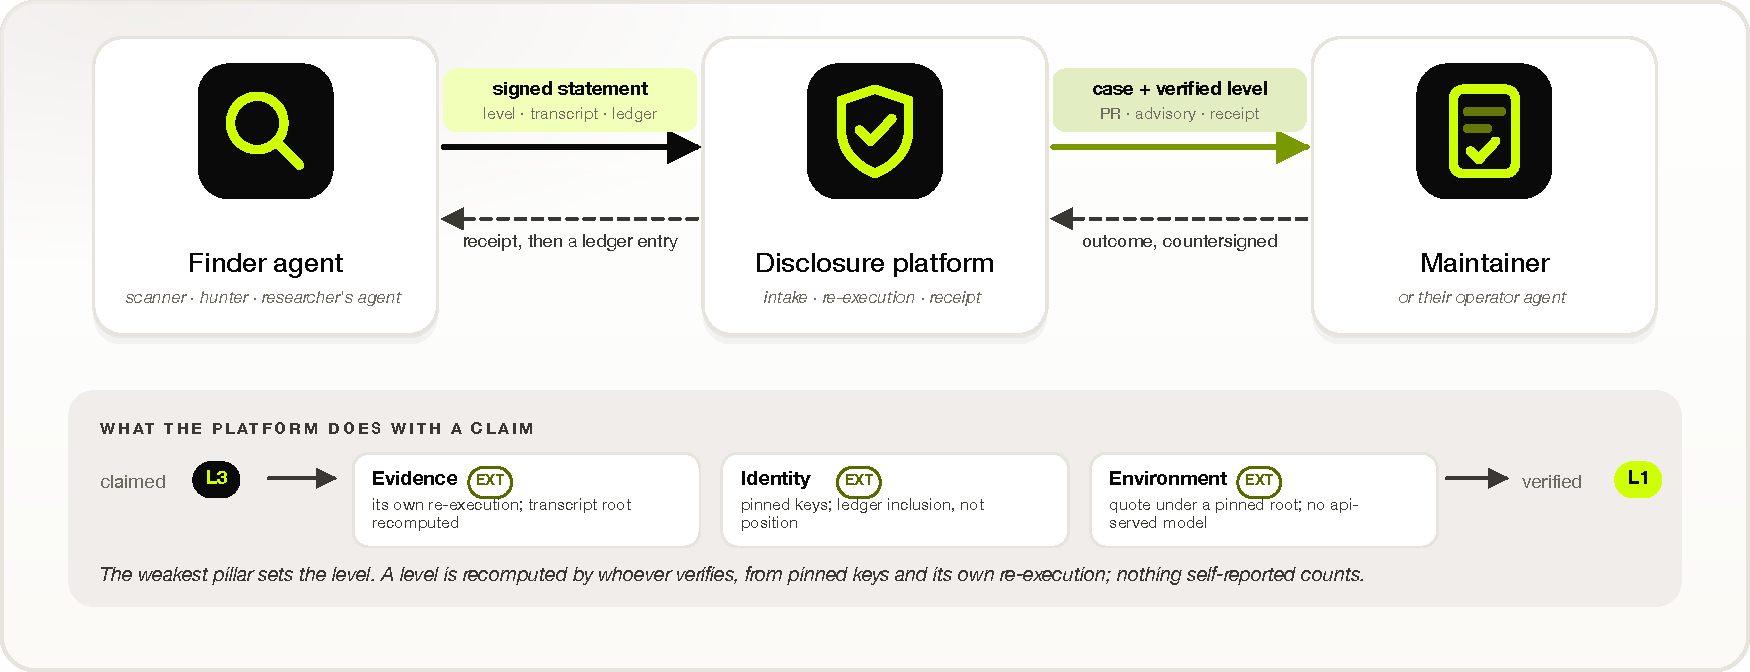
\includegraphics[width=0.96\linewidth]{../figures/pdf/fig-cover.pdf}
\end{center}
\vspace{0.4em}

\noindent
\glance{teal}{Pillars, levels, tracks}{Evidence, Identity and Environment are asked of every disclosure; \lvl{0} Unattested to \lvl{3} Hardened; a Finding track and a Patch track. The weakest pillar sets the level.}\hfill
\glance{violet}{Claimed is not verified}{A receiver recomputes the level from pinned keys, expectations and its own re-execution. Every check is external or structural; nothing self-reported stands in for an input.}\hfill
\glance{ink}{Probed, not asserted}{Five reviews over three rounds attacked the verifier, rubric and ledger. Every attack is now a failing test; every threat is marked defeated, mitigated or recorded.}


\newpage

% ------------------------------------------------------------------ abstract page
\thispagestyle{empty}
\noindent{\footnotesize\sffamily\bfseries\color{teal}\MakeUppercase{Abstract}}\par
\vspace{0.3em}
\noindent
\begin{tikzpicture}\fill[aailime] (0,0) rectangle (2.2cm,0.09cm);\end{tikzpicture}
\vspace{0.8em}

\noindent\begin{minipage}{\textwidth}
{\linespread{1.06}\selectfont
Coordinated vulnerability disclosure (CVD) was designed for people with inboxes: a researcher writes to a
security address, a maintainer reads it, and a 90-day clock gives the maintainer time to fix the bug before
it is published. Both ends of that process are now increasingly machines. Scanners, fuzzers and research
agents produce findings at machine speed; maintainers increasingly answer with agents that triage, reproduce,
patch and publish. What is missing is a way for the receiving machine to know how far to trust the sending
one. We propose \vsla{} (Vulnerability-disclosure Supply-chain Levels for Agents), a graded framework modelled
on \slsa{}. A disclosure carries a signed provenance statement that binds the finding to the exact code, to a
model bill of materials, to a Merkle-rooted transcript of every model turn and tool call, and to a reproduction
that was executed by code rather than asserted by a model (\lvl{1}). A disclosure platform re-executes the
reproduction itself, countersigns a receipt, and verifies the finder's countersigned trust ledger against the
countersigners it has pinned (\lvl{2}). At the top, the model weights, harness and signing key live in an
attested environment, so the statement is attributable to a measured run (\lvl{3}). None of the primitives are new: signed in-toto statements, Merkle-logged agent runs, attested inference and agent
reputation ledgers all exist. What is new is their composition into graded, verifiable levels for the disclosure
itself, with reproduction-by-code and receiver re-execution as the evidence rule that separates the levels. We
give the threat model, with each threat marked as defeated, mitigated or merely recorded at its level; the
provenance format; a verification procedure that distinguishes a \emph{claimed} level from a \emph{verified} one
and an external check from a structural one; a trust rubric and the attacks its first version was shown to
permit; an open-source implementation in qudisclose; a survey of what already exists and where the gaps are;
and the shape of the pilots we are arranging with partner projects, which will measure whether attested machine
patches are accepted more often, and no less safely, than unattested ones. This is the fourth draft: five adversarial reviews over three rounds probed the artefacts rather than reading the
prose, each found the verifier granting something it had not checked, and every attack they demonstrated is now a
failing test.
\par}
\end{minipage}

\vspace{0.7em}
\noindent{\footnotesize\sffamily\bfseries\color{violet}\MakeUppercase{A reader's guide}}\par
\vspace{0.3em}
\noindent
\begin{tikzpicture}\fill[aailime] (0,0) rectangle (2.2cm,0.09cm);\end{tikzpicture}
\vspace{0.6em}

\noindent\begin{minipage}[t]{0.47\textwidth}\footnotesize
\begin{description}[leftmargin=0pt, labelsep=0.5em, itemsep=0.25em, font=\normalfont\bfseries]
  \item[1--3 \, Why, and what already exists.] Human CVD meets machine finders; \slsa{}, in-toto, DSSE, TEEs and transparency logs; what each primitive already does and what this paper adds (Table~\ref{tab:related}).
  \item[\ref{sec:threats} \, What goes wrong.] Twenty-five threats, each marked \emph{defeated}, \emph{mitigated} or \emph{recorded} at a level (Figure~\ref{fig:threats}). Start here if you are a maintainer.
  \item[\ref{sec:framework} \, The framework.] Three pillars, four levels, two tracks, and the rule that the weakest pillar sets the level.
  \item[\ref{sec:provenance} \, Provenance.] The statement, the receipt, the ledger and the quote: digests go in, bodies stay out. Start here if you will implement it.
\end{description}
\end{minipage}\hfill
\begin{minipage}[t]{0.47\textwidth}\footnotesize
\begin{description}[leftmargin=0pt, labelsep=0.5em, itemsep=0.25em, font=\normalfont\bfseries]
  \item[\ref{sec:verification} \, Verification and the rubric.] How a claimed level becomes a verified one, which checks are external, and the score within a level. Start here if you will verify.
  \item[\ref{sec:impl} \, Implementation.] qudisclose as finder and platform (Figure~\ref{fig:qudisclose}).
  \item[\ref{sec:pilots} \, Pilots.] What will be measured, paired with the safety metrics that keep ``merged faster'' honest.
  \item[\ref{sec:discussion} \, Discussion.] Trust the badge, ledgers instead of bounties, the provider's asymmetric risk, and the limits this paper inherits and leaves.
\end{description}
\end{minipage}

\vfill
\noindent{\color{aaineutral}\rule{\textwidth}{0.6pt}}\\[0.4em]
{\footnotesize\itshape The idea in one sentence: a statement claims a level; a receiver recomputes it from pinned keys, expectations and its own execution, and the weakest pillar wins.}

\newpage
\setcounter{page}{1}


\section{Introduction}

The median time from report to fix in open source is measured in weeks, and for a solo maintainer the latency
\emph{is} the vulnerability window. The disclosure norms that produce that latency were reasonable when a
report was a rare, hand-written thing. They are not reasonable when a self-hosted model on two desktop machines
can produce a reproducible finding every few minutes, nor when the maintainer's side of the conversation is
also a model.

The qudisclose project~\cite{qudisclose} is one instance of the new shape: a researcher's agent submits a
report over the Model Context Protocol, a team of agents acknowledges in seconds, reproduces, patches,
reviews, publishes, and writes the postmortem, with a 7-day embargo cap instead of 90 and the embargo ending the
moment the fix ships. Building it exposed a question the human process never had to answer precisely:
\emph{on what basis should one machine believe another machine's claim that a bug exists, that a model found
it, that the account of how it was found is complete, and that the fix is correct?} The human process answered
with reputation, email headers and good faith. None of those survive contact with a thousand findings a day.

Software builds faced the same question a few years ago, and the answer was \slsa{}: a ladder of levels, each
a floor of requirements on provenance, platform and verification, so that a consumer can state in one word
how much a build artifact can be trusted and a producer knows what it must do to earn the next word.
\vsla{} applies that design to disclosures. It is deliberately small: three pillars, three levels above zero,
two tracks, one provenance predicate, one verification procedure, one score.

\paragraph{What is and is not new.}
We want to be precise about the claim, because every primitive in \vsla{} exists elsewhere and a reader who
knows the supply-chain literature will recognise each one. Signed in-toto statements for AI-produced code are
being standardised now~\cite{intoto604,attestproj}; Merkle-logged, DSSE-signed agent runs exist~\cite{flightrecorder,novafabric,vct};
model inference attested in a TEE and written to a consistency-proofed log exists~\cite{teegrant}; reputation
ledgers for agents are proposed~\cite{agentreputation,zer0n}; and a \slsa{}-style tiering has been applied to
agent skill packages~\cite{skillslsa}. Section~\ref{sec:related} goes through each. What we could not find, and
what this paper contributes, is:

\begin{enumerate}
  \item A graded trust framework for the \emph{disclosure} rather than for the code, the agent or the run, with separate Finding and Patch tracks (Section~\ref{sec:framework}), and a threat model for machine-to-machine disclosure (Section~\ref{sec:threats}) that names the attacks the human process has no vocabulary for: cherry-picked transcripts, substituted models, forged provenance, tampered weights, and a model provider's asymmetric knowledge.
  \item The evidence rule that separates the levels: a finding's evidence is a test \emph{executed by code} that fails by assertion at the subject revision, and \lvl{2} requires that the \emph{receiver} re-executed it, classified it and checked that it loaded the code it names. The ``AI slop'' literature describes the problem and proposes a score for polish versus substance~\cite{slopsurvey}; we make execution a mechanical, signable requirement, and say plainly that it proves reproducibility, not validity.
  \item A provenance predicate (Section~\ref{sec:provenance}) that puts a model bill of materials in every disclosure, so a bad model can be traced to every finding it touched, and that commits to the transcript with a Merkle tree so a single turn can be proven without releasing the prompts.
  \item The platform \emph{receipt}, a separate countersignature over statement digest, channel, time and the platform's own re-execution, review and scope result, which counts only under the platform key the statement itself names and which a third-party verifier requires to be anchored by log inclusion; and a trust ledger whose index its owner assigns, whose entries are countersigned by the party that bore the cost of the report, bound to the finder's key and to the track, and count only with readers who have pinned that party, which is what lets a ledger replace a bounty without becoming a forgeable or transferable credential.
  \item A verification procedure (Section~\ref{sec:verification}) in which a claimed level is recomputed by the receiver from what it can check against its own pinned keys and expectations, every check is marked external or structural, every time-dependent check is judged at one instant fixed by the anchor rather than by the party being checked, a self-reported value never substitutes for an input, and a coordinator without the code lands, honestly, at \lvl{1}.
  \item An implementation (Section~\ref{sec:impl}) in qudisclose that produces and verifies statements on both tracks, a reference verifier with signed examples on both tracks at every level that is byte-compatible with it, and the evaluation we are arranging with pilot partners (Section~\ref{sec:pilots}), whose metrics pair acceptance and time-to-merge with revert rate and adversarial false acceptance.
\end{enumerate}

\section{Background}

\paragraph{Coordinated vulnerability disclosure.}
ISO/IEC 29147 and 30111~\cite{iso29147,iso30111} and the CERT guide~\cite{certcvd} describe CVD as a human
workflow: receipt, acknowledgement, triage, remediation, release, with an embargo whose canonical length,
90 days, comes from Project Zero's policy~\cite{p0}. The pathologies are well known: slow acknowledgement,
disputes over who found what first, early embargo breaks when parties disagree about evidence of exploitation,
and fixes released through non-authoritative channels that dependents cannot pull from the distribution they
already trust. Bounties fix some incentives and break others; core-infrastructure maintainers have declined
bounty programs because of the arguments they generate over breaking fixes and the distortion of volunteer
pipelines.

\paragraph{\slsa{}, in-toto and DSSE.}
\slsa{}~\cite{slsa} defines Build levels \lvl{1} (provenance exists), \lvl{2} (signed by a hosted platform) and
\lvl{3} (hardened, isolated builder whose provenance is non-forgeable). Provenance is an in-toto
Statement~\cite{intoto} in a DSSE envelope~\cite{dsse}; the consumer verifies rather than trusts. \slsa{}
v1.0 split its requirements into tracks (Build; Source in progress) when it became clear that one ladder could
not express two independent claims. \vsla{} borrows all of this.

\paragraph{Models as supply-chain components.}
A model is a dependency of a finding in the way a library is a dependency of a build. The software bill of
materials has a model analogue (CycloneDX ML-BOM~\cite{cyclonedx}); model signing is being standardised
under OpenSSF~\cite{modelsigning}; backdoored and sleeper fine-tunes are a demonstrated risk~\cite{sleeper};
and quantization changes model behaviour in ways that are rarely attested. Trusted execution environments
(AMD SEV-SNP~\cite{sevsnp}, Intel TDX~\cite{tdx}) attest a measurement of what is running to a remote party;
a two-operator split obtains a TEE-like guarantee without a chip vendor by secret-sharing across two
independently owned hosts with a 2-of-2 signing group and cross-diffed Merkle logs. Transparency logs
(RFC 6962~\cite{rfc6962}, Sigstore~\cite{sigstore}, IETF SCITT~\cite{scitt}) give append-only, auditable
records with inclusion and consistency proofs.

\paragraph{Secure agent plumbing.}
The NSA's 2026 guidance on MCP security design~\cite{nsamcp} treats the model, client, server and tools as
one trust domain and asks for per-message integrity, least privilege at the tool boundary, no long-lived
credentials in agent context, distinct non-human identities, tamper-evident audit of inputs and outputs, and
tool output treated as untrusted input. qudisclose implements the ones a disclosure intake needs (per-message
signed envelopes with nonces, scoped bearer tokens, a hash-chained signed audit log, strict input models, tool
output treated as untrusted); \vsla{} assumes them and builds the disclosure-specific layer on top.

\section{Related work, and the gaps \vsla{} fills}
\label{sec:related}

\paragraph{Provenance for AI-produced code.}
The in-toto attestation project has an open proposal to register a predicate for AI code-generation provenance
that records which line ranges a model produced, which model and agent produced them, and a hash of the prompt
rather than its text~\cite{intoto604}, alongside pending predicates for change authorship and review at the
pull-request level and for agent actions and decisions. A small project named \emph{attest} already produces
signed, tamper-evident provenance for AI-assisted changes with in-toto, DSSE and Sigstore~\cite{attestproj}.
These answer ``which model wrote these lines''; \vsla{} reuses their formats and asks the next question,
``should I believe this bug is real and this fix is right''. Our Patch track could carry the line-range
predicate as a companion statement, and our predicate should be registered in the same place.

\paragraph{Tamper-evident agent runs.}
Agent Flight Recorder hash-chains per-event records and batches them into Merkle epochs with inclusion proofs,
and names TEE-attested completeness as future work~\cite{flightrecorder}. NovaFabric records an agent run into an
append-only Merkle log with a redaction attestation, signed with DSSE and trusted timestamps, as provider-neutral
evidence whose post-hoc changes are detectable~\cite{novafabric}. VCT handles the branching that LLM conversations
produce (edits, regeneration) with per-branch chains rolled into session roots~\cite{vct}, and MemMark signs a
per-session Merkle root over per-decision commitments~\cite{memmark}. \vsla{}'s transcript commitment is the same
technique; its contribution is only to make the commitment a required field of a disclosure and to specify which
leaf (the code-side verification step) a verifier must find in it.

\paragraph{Attested inference.}
Running model evaluation inside a TEE, checking the attestation chain to the hardware root, verifying that the
measurement matches an approved model and prompt, and appending the attested bundle to a consistency-proofed log
has been built for AI-assisted grant evaluation~\cite{teegrant}. \vsla{} \lvl{3} is that design applied to a finder,
with the signing key bound by the quote. Two caveats from that literature carry over unchanged: a TEE will run
whatever code it is given and an audit trail will record whatever the agent does, so neither establishes that
the agent's intent was legitimate~\cite{aiidentity}; and attestation binds execution to a code hash but does
not by itself show the code satisfies a trust property~\cite{cryptoai}. \vsla{} does not claim otherwise; its
levels are about tamper-evidence and attributability, and the \emph{receiver's} re-execution is what speaks to
correctness.

\paragraph{Agent identity and reputation.}
Zero-trust identity designs give agents decentralised identifiers as anchors for accumulating
reputation~\cite{zerotrustagent}, and a 2026 survey of AI identity standards separates an agent's own
provenance from the provenance of what it produces, noting that provenance shows where an agent came from but
not why it acts as it does~\cite{aiidentity}. AgentReputation proposes separating task execution, reputation
computation and tamper-proof storage, keeps per-task reputation so that low-stakes evidence cannot inflate trust
in high-stakes tasks, and lists cold-start bootstrapping and manipulation resistance as open
problems~\cite{agentreputation}. Zer0n anchors AI-assisted vulnerability assessments to a blockchain and leaves
reputation tied to on-chain history as future work~\cite{zer0n}. \vsla{}'s ledger differs in one respect that we
think is decisive: entries are countersigned by the maintainer or platform that received the disclosure and paid
the cost of checking it, not self-reported or computed by a third party. That is what makes it a substitute for a
bounty, and it addresses AgentReputation's per-task concern directly, since a \vsla{} ledger is per track.
Cold start is handled by design rather than solved: a new finder is \lvl{1} until it earns \lvl{2}.

\paragraph{The slop problem.}
Maintainers triaging Node.js and enterprise open-source report a flood of plausible, unverified AI-generated
vulnerability reports whose submitters do not know they are fake~\cite{herodevs}; a survey formalises ``AI
slop'' as automatically generated security artifacts and proposes a Slop-Score for the gap between polish and
verifiable substance~\cite{slopsurvey}; and the Cloud Security Alliance notes that when bounties become
economically unviable, open-source maintainers lose their main channel for outside reports~\cite{csadisclosure}.
The same period produced the counter-example: AI tooling found and upstreamed every CVE in one curl release,
all accepted by the maintainers~\cite{herodevsguide}. \vsla{} is the mechanism that lets a maintainer tell those
two cases apart before reading the report, because the second one can carry a failing test re-run by code and
the first cannot.

\paragraph{\slsa{}-style tiers for agent artifacts.}
A graduated model that maps trust scores to four levels, from unsigned to formally verified, and lets enterprise
policy require a minimum level has been proposed for agent \emph{skill} packages~\cite{skillslsa}. It is the
nearest precedent for applying \slsa{}'s shape to an agent-era artifact. We know of no such tiering for findings
or patches. A caution from the authorisation literature applies to both: a signed attestation establishes
provenance, and none of these attestations should automatically count as proof that requirements were met or
that a system is safe~\cite{agentoutput}. In \vsla{} that is why a level is a statement about evidence and
attributability, never a merge decision.

\begin{table}[htbp]
\small\centering
\begin{tabular}{p{0.3\linewidth}p{0.33\linewidth}p{0.3\linewidth}}
\toprule
\textbf{Component} & \textbf{Already exists} & \textbf{What \vsla{} adds} \\
\midrule
Signed provenance for AI output & in-toto AI predicates~\cite{intoto604}, attest~\cite{attestproj} & a predicate for the \emph{disclosure}: finding, fix, MBOM, reproduction \\
Merkle-logged agent runs & \cite{flightrecorder,novafabric,vct,memmark} & required in every statement; the verification leaf a verifier must find \\
Attested inference & \cite{teegrant} & the \lvl{3} Environment pillar; key bound by the quote; two-host option \\
Agent reputation & \cite{agentreputation,zer0n,zerotrustagent} & countersigned by the receiver; per track; replaces the bounty \\
Graded trust levels & \slsa{}~\cite{slsa}; skills~\cite{skillslsa} & levels for findings and patches; weakest pillar; claimed vs verified \\
Slop detection & Slop-Score~\cite{slopsurvey} & substance as a mechanical requirement: a test re-run by code, then by the receiver \\
\bottomrule
\end{tabular}
\caption{What \vsla{} reuses and what it adds.}
\label{tab:related}
\end{table}

\section{What goes wrong with a machine disclosure}
\label{sec:threats}

\begin{figure}[htbp]
  \centering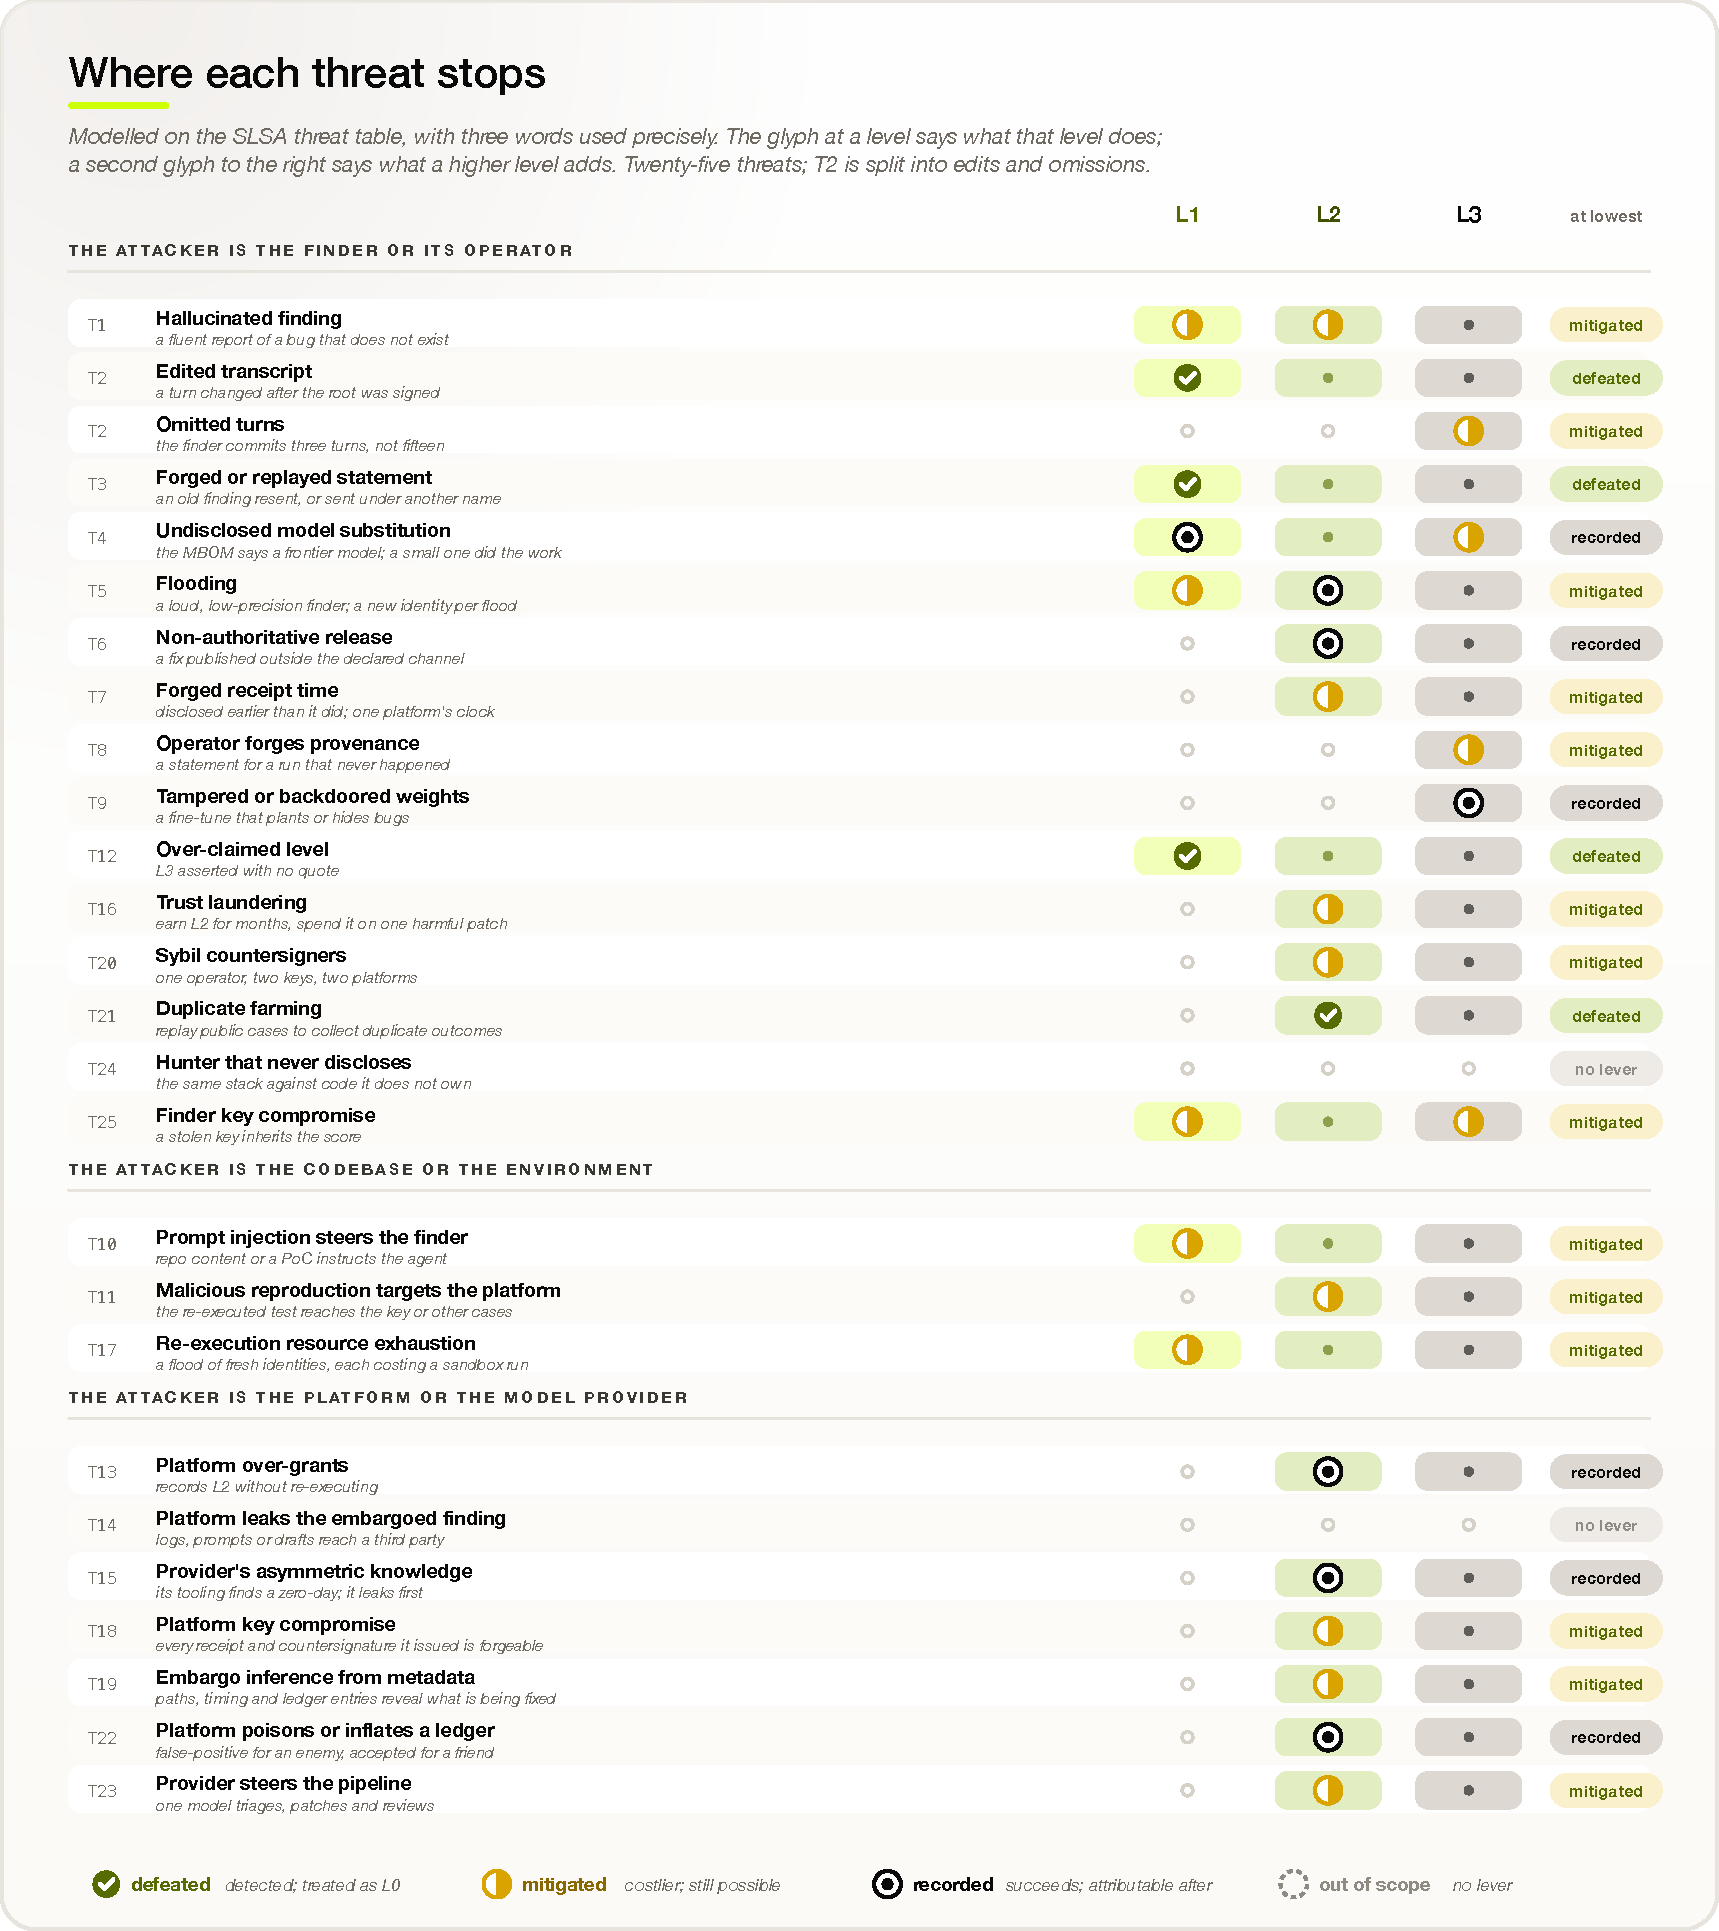
\includegraphics[width=0.88\linewidth]{../figures/pdf/fig-threats.pdf}
  \caption{Where each threat stops. The glyph at a level says what that level does against the threat: \emph{defeated} (detected mechanically, the disclosure is treated as \lvl{0}), \emph{mitigated} (costlier, still possible) or \emph{recorded} (it succeeds and is attributable afterwards); a second glyph to the right says what a higher level adds. Twenty-five threats; T2 is split into edits and omissions. The specification's table carries the residuals.}
  \label{fig:threats}
\end{figure}

Figure~\ref{fig:threats} is the framework's threat table in the \slsa{} style, with one discipline \slsa{}'s table
does not need: three distinct words for what a level does. The first draft of this paper said ``defeated'' in
rows where only ``mitigated'' or ``recorded'' is true, and two reviewers caught it independently. A level
\emph{defeats} a threat when the receiver detects it mechanically and treats the disclosure as \lvl{0} before
acting. It \emph{mitigates} a threat when it raises the cost or narrows the attack, which can still succeed. It
\emph{records} a threat when the attack succeeds and the level makes it attributable to an identity afterwards.
Most of what \vsla{} does is the second and third kind, and a framework that claims otherwise is the thing it
was built to prevent.

\paragraph{The finder or its operator.} A \emph{hallucinated finding} (T1) is a fluent report of a bug that
does not exist; its cost is an hour of a maintainer's attention, and at scale it is the whole alert-fatigue
problem. \lvl{1} mitigates it by requiring a test that was executed, which removes reports that were never run;
\lvl{2} mitigates it further by having the receiver run the test itself, classify the failure with its own
classifier and check that the test loaded the package the receiver's own configuration names. Neither defeats it:
a finder can write a test that fails on demand, \texttt{import subject; assert False} clears both checks, and the
runner's report that the classifier reads is written inside the process the hostile test runs in; the classifier
filters honest error, and \lvl{1} proves reproducibility, not validity. An \emph{edited transcript} (T2)
is defeated at \lvl{1} by the Merkle root, but a transcript with turns \emph{omitted} before the root was signed
is invisible to any root; only a recorder inside a measured harness (\lvl{3}) can attest completeness, and the
figure lists the two separately. A \emph{forged or replayed statement} (T3) and an \emph{over-claimed level}
(T12) are defeated at \lvl{1}. \emph{Model substitution} (T4) is recorded at \lvl{1} (the MBOM is signed) and
mitigated at \lvl{3} (the quote binds the weights that ran); an API-served model is unmeasurable at every level.
\emph{Flooding} (T5) is mitigated at \lvl{1} by admission control on what an unknown identity can make the
platform execute, and recorded at \lvl{2} by the ledger. \emph{Non-authoritative release} (T6) is recorded at
\lvl{2}; nothing prevents a leak. A \emph{forged receipt time} (T7) is mitigated at \lvl{2}, and only mitigated:
a receipt is one platform's clock unless it is anchored in a transparency log, and in the qudisclose
configuration the platform and the finder can be the same operator. \emph{Forged provenance} (T8) is mitigated at
\lvl{3}: the key cannot leave the enclave, but the operator still chooses the enclave's inputs. \emph{Tampered
weights} (T9) are recorded at \lvl{3}: attestation names the bytes, not their behaviour.

Three threats the first draft did not have come from the long game and the ledger. \emph{Trust laundering}
(T16) is the xz-utils pattern with a reputation ledger in place of a human persona: a finder earns \lvl{2} over
months and spends it on one harmful change, a weakened check or a payload in a fixture. \vsla{} mitigates it at
\lvl{2} with three rules: the receiver runs its own review on a model family different from the patcher's; a
diff that touches build scripts, CI, fixtures, binaries, manifests or release tooling is capped at \lvl{1}
whatever the review says, because that is where real compromises have landed; and a patch reverted for cause
is a disqualifying, retroactive outcome. None of that makes a source-only diff safe to merge unread, and the
paper says so where it matters (Section~\ref{sec:discussion}). \emph{Sybil countersigners} (T20) are one
operator running two keys and two platforms, or a finder presenting another finder's published ledger as its own;
the defence is that a verifier counts only countersigners it has pinned, per operator, that every entry is bound to
the finder's key and the track it was earned on, and a hard age gate on the floor. \emph{Duplicate farming} (T21), replaying public cases to collect
positive outcomes, is defeated by making duplicates neutral in the rubric. A \emph{compromised finder key}
(T25) inherits the finder's score; validity windows, revocation entries and anchored receipts are the
mitigation.

\paragraph{The codebase or the environment.} \emph{Prompt injection} (T10): a comment in the repository tells
the agent to report nothing, or a proof-of-concept in a report tells the triage agent to rate it critical.
Mitigated at \lvl{1}, eliminated at none. A \emph{malicious reproduction} (T11) is the threat the first draft
listed as ``sandbox escape'' and marked defeated by policy. It is the largest exposure in the design: \lvl{2}
\emph{requires} the platform to execute a test written by a party it has no history with, and the platform's
signing key is the whole of \lvl{2}. The specification now states isolation requirements (no egress, no access
to keys, tokens, the database or other cases, resource caps, a distinct principal, VM isolation in production,
the isolation class written into every receipt) and admission control (T17); the threat is mitigated, and a
platform running a process-level sandbox in production has not mitigated it.

\paragraph{The platform or the model provider.} A platform may \emph{over-grant} a level (T13), \emph{leak} an
embargoed finding (T14), \emph{poison or inflate} a ledger (T22), or have its \emph{key stolen} (T18), which
forges every receipt and countersignature it ever issued. \emph{Embargo inference} (T19) reads which projects
are being probed, which files, and when the fix is coming from statement fields, ledger timing and status
polling; the first draft called the statement ``safe to publish while embargoed'' while its predicate carried
the test path, the command and the files touched in plaintext. The embargoed profile and a rule that no
per-case metadata is exposed until the case is public are the mitigation. A model provider with advanced
internal tooling has \emph{asymmetric knowledge} (T15), and a platform that runs every role on one provider's
model has that provider \emph{steering} every decision (T23); reviewer diversity on the Patch track is the only
structural defence. Finally, a \emph{hunter that never discloses} (T24) is out of scope by construction and
listed so that nobody mistakes the omission for an oversight: \vsla{} does not reduce what an autonomous
hunter can do, and every lever it has acts on an identity that submits statements.

\section{The framework}
\label{sec:framework}

\begin{figure}[htbp]
  \centering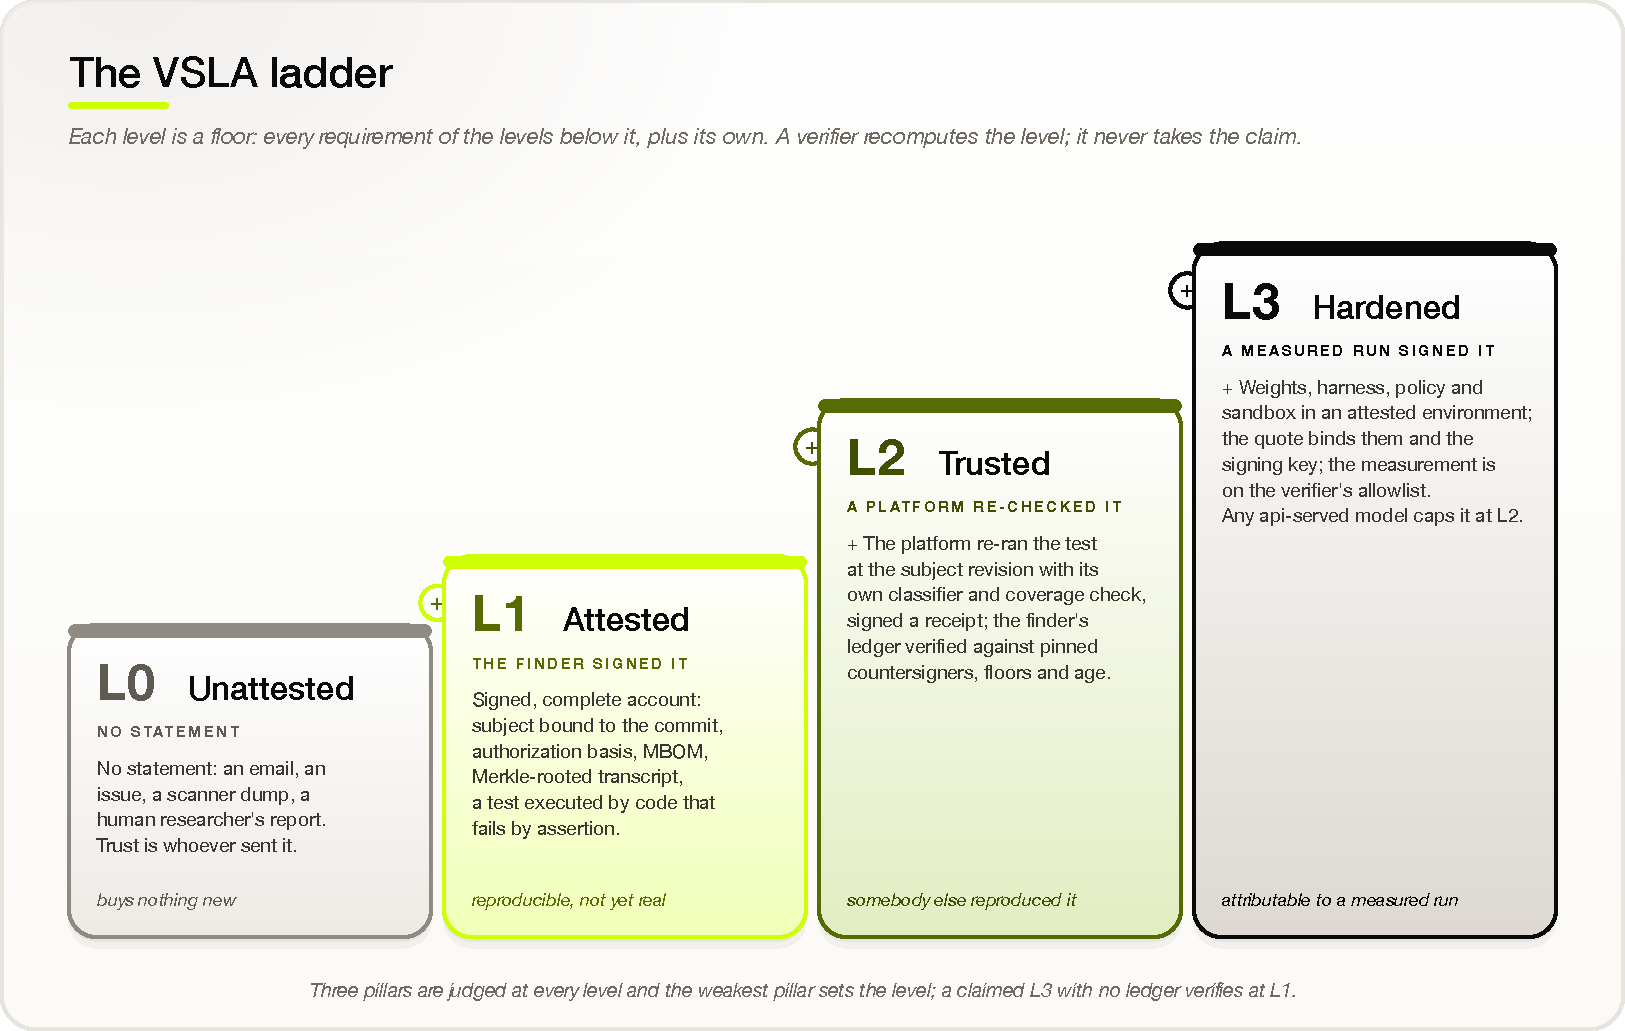
\includegraphics[width=\linewidth]{../figures/pdf/fig-ladder.pdf}
  \caption{The \vsla{} ladder. Each level is a floor: all requirements of lower levels plus its own.}
  \label{fig:ladder}
\end{figure}

\vsla{} has four levels (Figure~\ref{fig:ladder}), three pillars, two tracks, and one rule for combining them:
a level is granted only when every pillar meets it, so the weakest pillar sets the level.

\subsection{Pillars}

\begin{figure}[htbp]
  \centering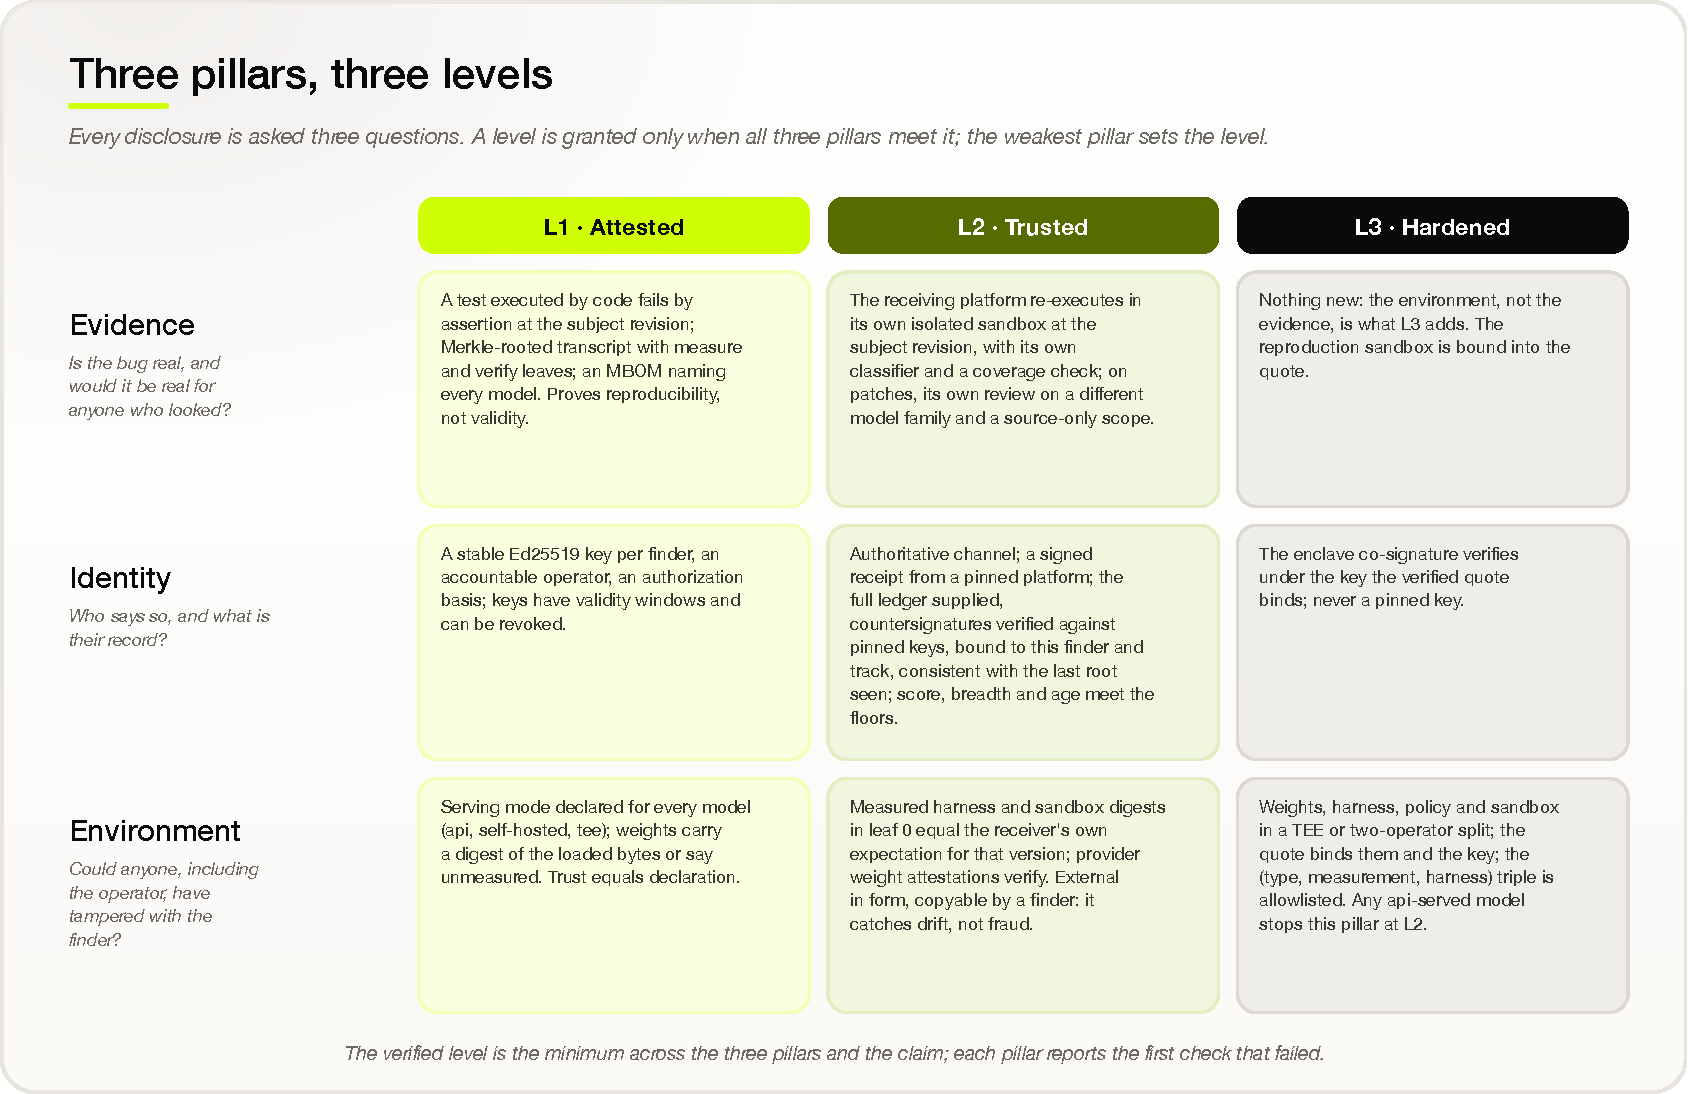
\includegraphics[width=\linewidth]{../figures/pdf/fig-pillars.pdf}
  \caption{The pillar-by-level matrix. A level is granted only when every pillar meets it.}
  \label{fig:pillars}
\end{figure}

Three questions are asked of every disclosure, and each pillar answers one (Figure~\ref{fig:pillars}).
\textbf{Evidence}: is the bug real, and would it be real for anyone who looked? Its material is the executable
reproduction, the transcript commitment and the model bill of materials. \textbf{Identity}: who says so, and
what is their record? Its material is the finder key, the operator, the authorization basis, the
authoritative channel and the trust ledger. \textbf{Environment}: could anyone, including the operator, have
tampered with the finder? Its material is the serving mode, the measured harness, attested weights, and an
enclave or two-operator split. Separating the pillars is what lets a verifier say precisely why a claimed
\lvl{3} verified as \lvl{1}: the evidence was fine, the ledger was not supplied, the environment had nothing to
compare against.

Every verification check is also marked \emph{external} or \emph{structural}. An external check compares the
statement against something the finder did not write: a pinned key, an expectation the receiver obtained
independently, or the receiver's own execution. A structural check compares the statement against itself.
Only external checks separate the levels. The first draft's verifier had several \lvl{2} and \lvl{3} checks that
were structural (the finder's harness digest against the finder's own first leaf; the finder's weight digest
against the finder's own copy of a ``provider attestation''), which is the \slsa{} mistake of verifying
provenance without expectations; the distinction is now explicit in the procedure and in every verification
record.

\subsection{Levels}

\textbf{\lvl{0} Unattested} is everything that exists today: an email, an issue, a scanner dump. Its trust is the
trust already placed in the sender. A human researcher's report is \lvl{0} by definition, and a platform's policy
must not route it below machine \lvl{1} or \lvl{2} on the strength of the level alone: the level grades machine
evidence, not people.

\textbf{\lvl{1} Attested}: the finder signed a complete, reproducible account of what it did. The statement binds
the subject (report digest and exact code revision), the basis on which the finder was authorised to test that
code, a model bill of materials naming every model with serving mode and, for self-hosted models, either a
digest of the loaded weight bytes or an explicit \texttt{unmeasured}, a Merkle-rooted transcript whose first
leaf measures the harness and whose verification leaf records the test run, and a reproduction executed by
code at the subject revision: a test, the command, the exit code, and a classification of the failure by a
normative rule (at least one collected test failed by assertion; no collection, import, fixture or timeout
error). \lvl{1} buys the receiver a report it can reject mechanically if it is incomplete, replayed, or edited
after signing, and a test it can run with one command. It buys no reason to believe the bug is real: the
finder wrote the test and set the flag.

\textbf{\lvl{2} Trusted}: an authoritative platform received it, re-checked it, and the finder has a
countersigned record. The disclosure went to the channel the codebase declares; the platform re-executed the
reproduction in its own isolated sandbox at the subject revision, classified the failure with its own
classifier, checked that the test loaded the package the platform names for that repository, and signed a receipt
binding statement digest, channel, time and that result (Figure~\ref{fig:evidence}); on the Patch track the
platform also ran its own adversarial review on a different model family and computed that the diff touches source
only. The finder's trust ledger, an append-only log of past disclosures with countersigned outcomes, was supplied in
full: the platform verified the countersignatures it has pinned, dropped entries that name another key or another
track, checked that the ledger extends the one it was shown last time and includes every entry the platform itself
wrote, and recomputed the score against its floors, which include a minimum age. \lvl{2} buys a finding somebody other than the
finder reproduced, a finder with a record the platform can read, rate-limit and revoke, a cost on flooding and
a record of non-authoritative release, and a timeline that is as good as the platform's clock and better when
the receipt is anchored in a log. It buys no assurance about the model, no proof the transcript is complete,
and no licence to merge unread.

\textbf{\lvl{3} Hardened}: the finder ran where no one, including its operator, could reach in
(Figure~\ref{fig:tee}). Weights, harness, policy and reproduction sandbox were served from an attested
environment, a hardware TEE or a two-operator split co-signed by two distinct operators; the quote binds the
enclave key, the harness digest, every weight digest and the sandbox digest; the receiver holds an allowlist of
acceptable measurements for that harness; every weight digest matches a provider-signed attestation; and the
statement carries, beside the finder's pinned signature, a co-signature under a key generated inside the
environment and never exported, so a statement signed by the finder key alone verifies no higher than \lvl{2}. \lvl{3} buys \emph{attribution}: the statement is attributable to a measured
environment running named weights, so substitution, forged provenance and tampered weights become visible or
traceable. It does not buy an honest harness (the allowlist is where that judgement lives), honest inputs (the
operator still chooses what the enclave sees), or well-behaved weights (attestation names the bytes, not the
behaviour). An API-served model cannot be measured, so a pipeline with any API-served model, including the
one this paper's authors run for their patch agents, stops at \lvl{2} on the Environment pillar.

\paragraph{Where the \slsa{} analogy breaks.} The first draft said \lvl{3} ``is the same move \slsa{} Build
\lvl{3} makes''. It is not. \slsa{} Build \lvl{3} is non-forgeable because a \emph{third party}, the hosted build
platform, holds the signing key away from the producer. \vsla{} \lvl{2} is a receiver-side property with no
\slsa{} analogue (the consumer re-executes and countersigns), and \vsla{} \lvl{3} keeps the key in hardware the
\emph{producer} operates. The analogue of \slsa{}'s trusted builder would be a third-party finder-hosting
platform that holds the key; \vsla{} v1.0 does not define that environment type, and a reader who imports
\slsa{} \lvl{3}'s guarantee into \vsla{} \lvl{3} will over-trust it. The two-operator form is a third
trust statement again: ``neither of two operators alone'' rather than ``not the operator''.

\begin{figure}[htbp]
  \centering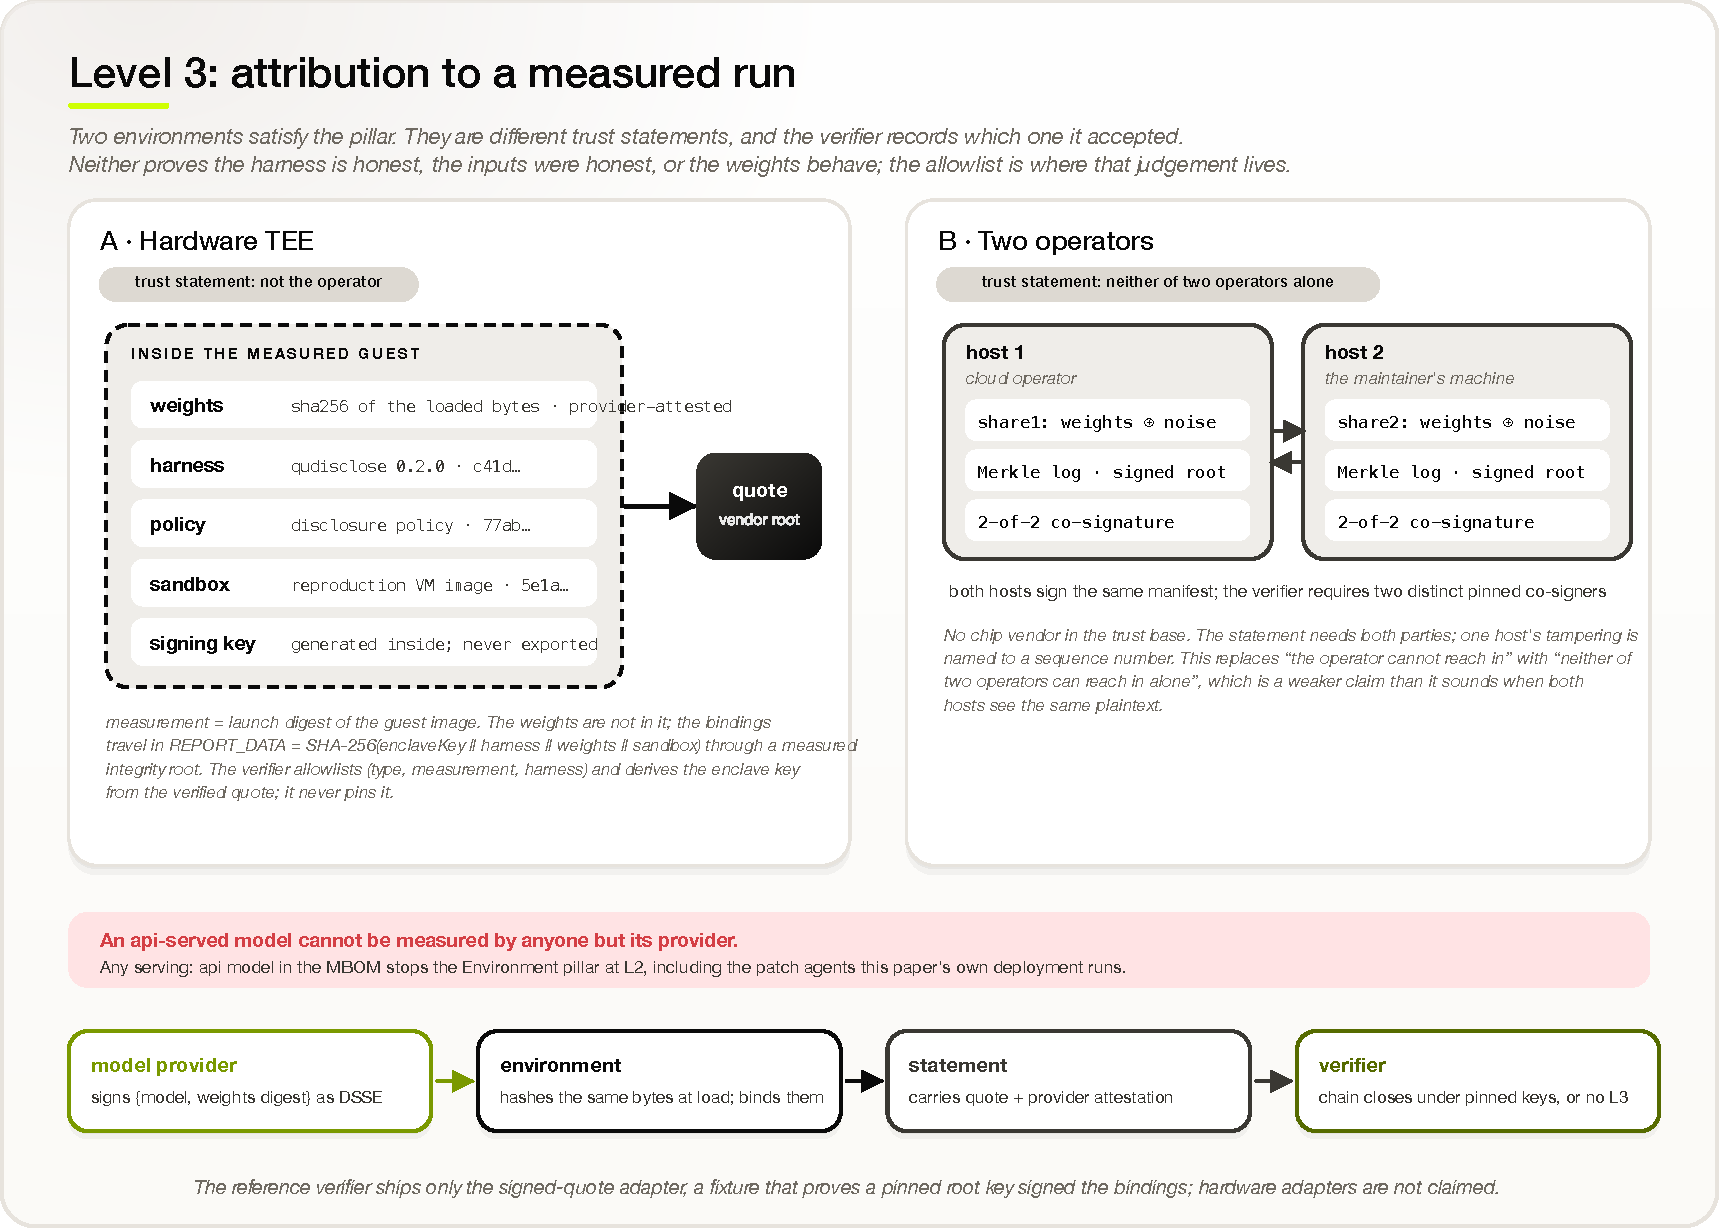
\includegraphics[width=\linewidth]{../figures/pdf/fig-tee.pdf}
  \caption{Two \lvl{3} environments. Either satisfies the Environment pillar; they are different trust statements (``not the operator'' and ``neither of two operators alone''), and a verifier records which one it accepted.}
  \label{fig:tee}
\end{figure}

\begin{figure}[htbp]
  \centering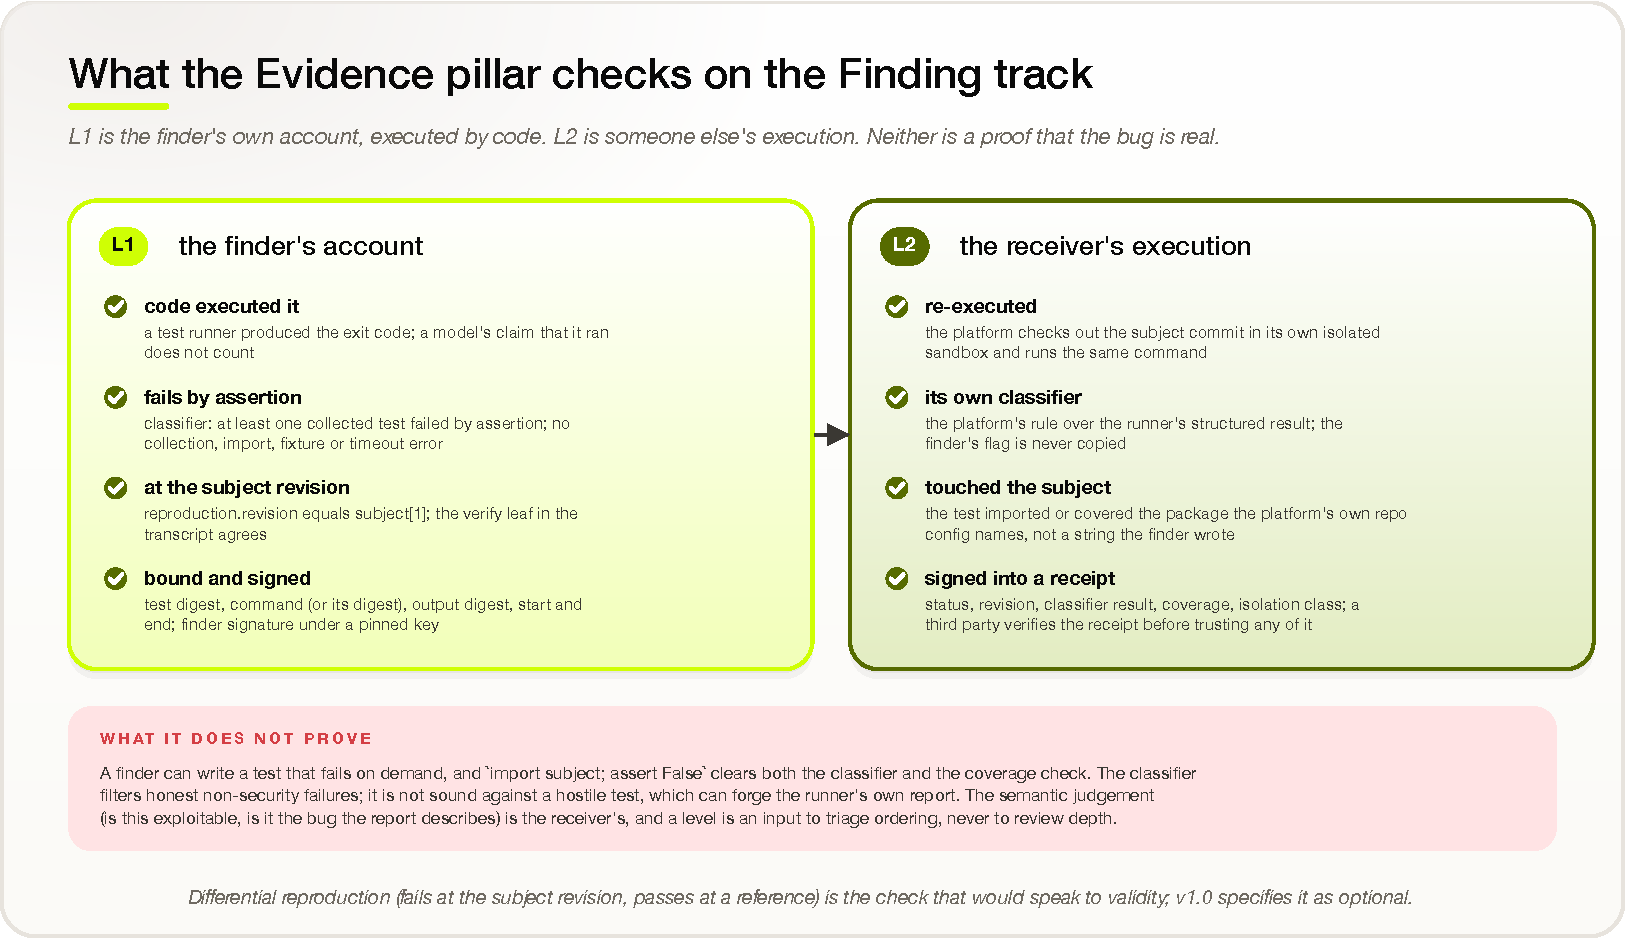
\includegraphics[width=\linewidth]{../figures/pdf/fig-evidence.pdf}
  \caption{What the Evidence pillar checks on the Finding track. \lvl{1} is the finder's own code-executed account; \lvl{2} is the receiver's re-execution at the subject revision with its own classifier and coverage check. Neither proves the bug is real: a finder can fail on demand, and the semantic judgement remains the receiver's.}
  \label{fig:evidence}
\end{figure}

\subsection{Tracks}

A disclosure makes two claims verified differently: \emph{this bug is real} and \emph{this fix is correct}.
\vsla{} keeps them on separate tracks with the same scale (Figure~\ref{fig:tracks}), so a receiver can say
``Finding \lvl{2}, Patch \lvl{1}'' and mean something precise, and ledger entries are scored per track so
precision on findings buys no trust on patches. The Patch track's \lvl{1} requires that the diff applied, the
reproduction passed and the project suite passed, all executed by code in a clean checkout, with the files
touched and a computed scope in the statement. Its \lvl{2} requires that the \emph{receiving platform} re-ran all
three, ran its own adversarial review on a model family different from every patcher in the MBOM, over the
diff and the test output only, and computed that the scope is source-only; a finder-asserted review satisfies
nothing. The Patch track answers the question maintainers actually ask of a machine patch, ``do I have to read
this carefully, or can I merge it?'', and the honest answer is narrower than the question: Patch \lvl{2} means
less review is needed to confirm that the fix closes the finding and passes the suite. It never means a change
to a security-sensitive surface may be merged unread.

\begin{figure}[htbp]
  \centering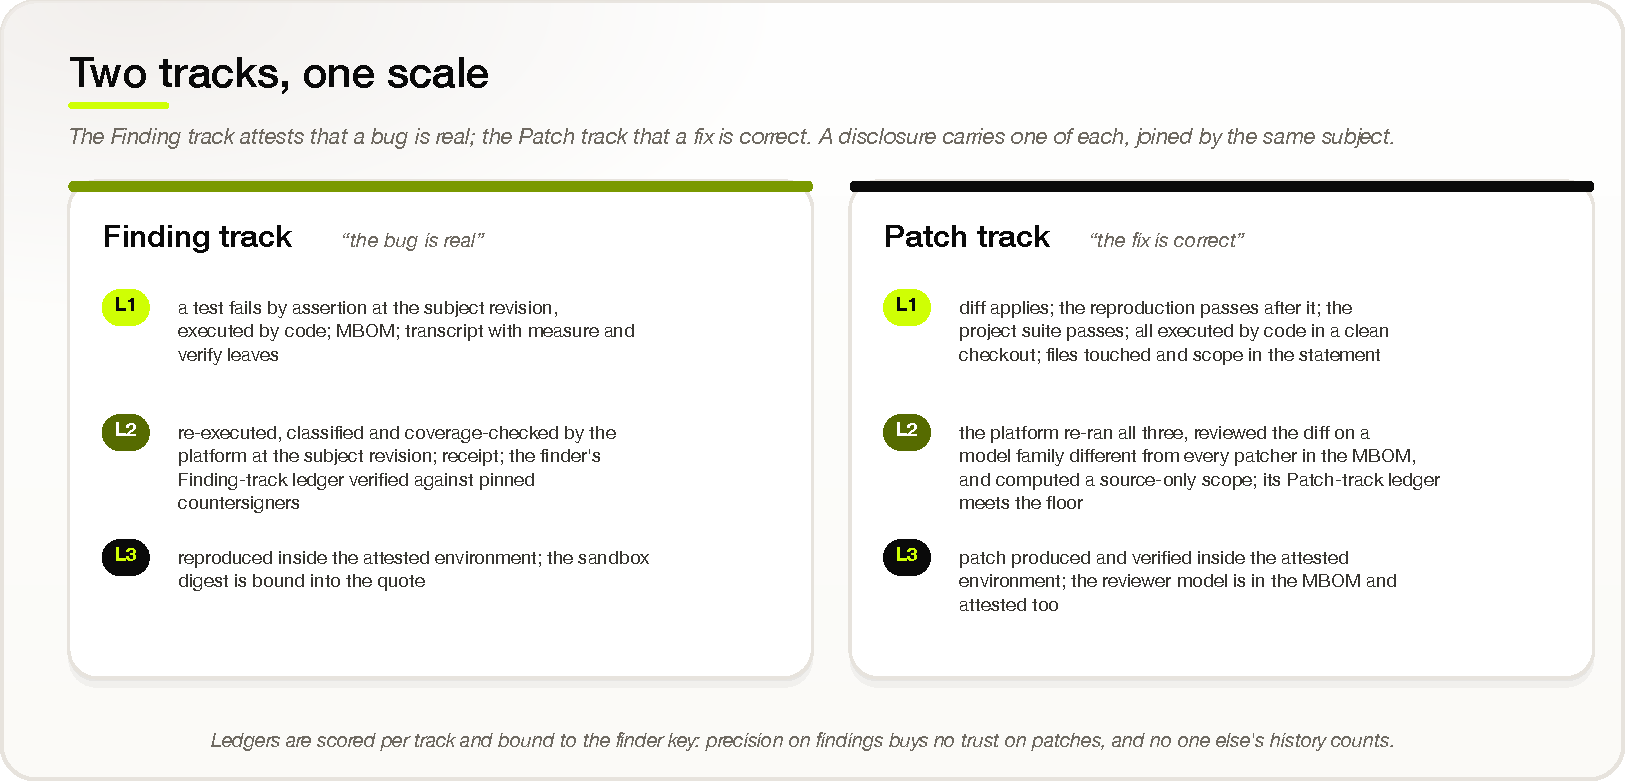
\includegraphics[width=\linewidth]{../figures/pdf/fig-tracks.pdf}
  \caption{The Finding and Patch tracks share one scale.}
  \label{fig:tracks}
\end{figure}

\section{Provenance}
\label{sec:provenance}

\begin{figure}[htbp]
  \centering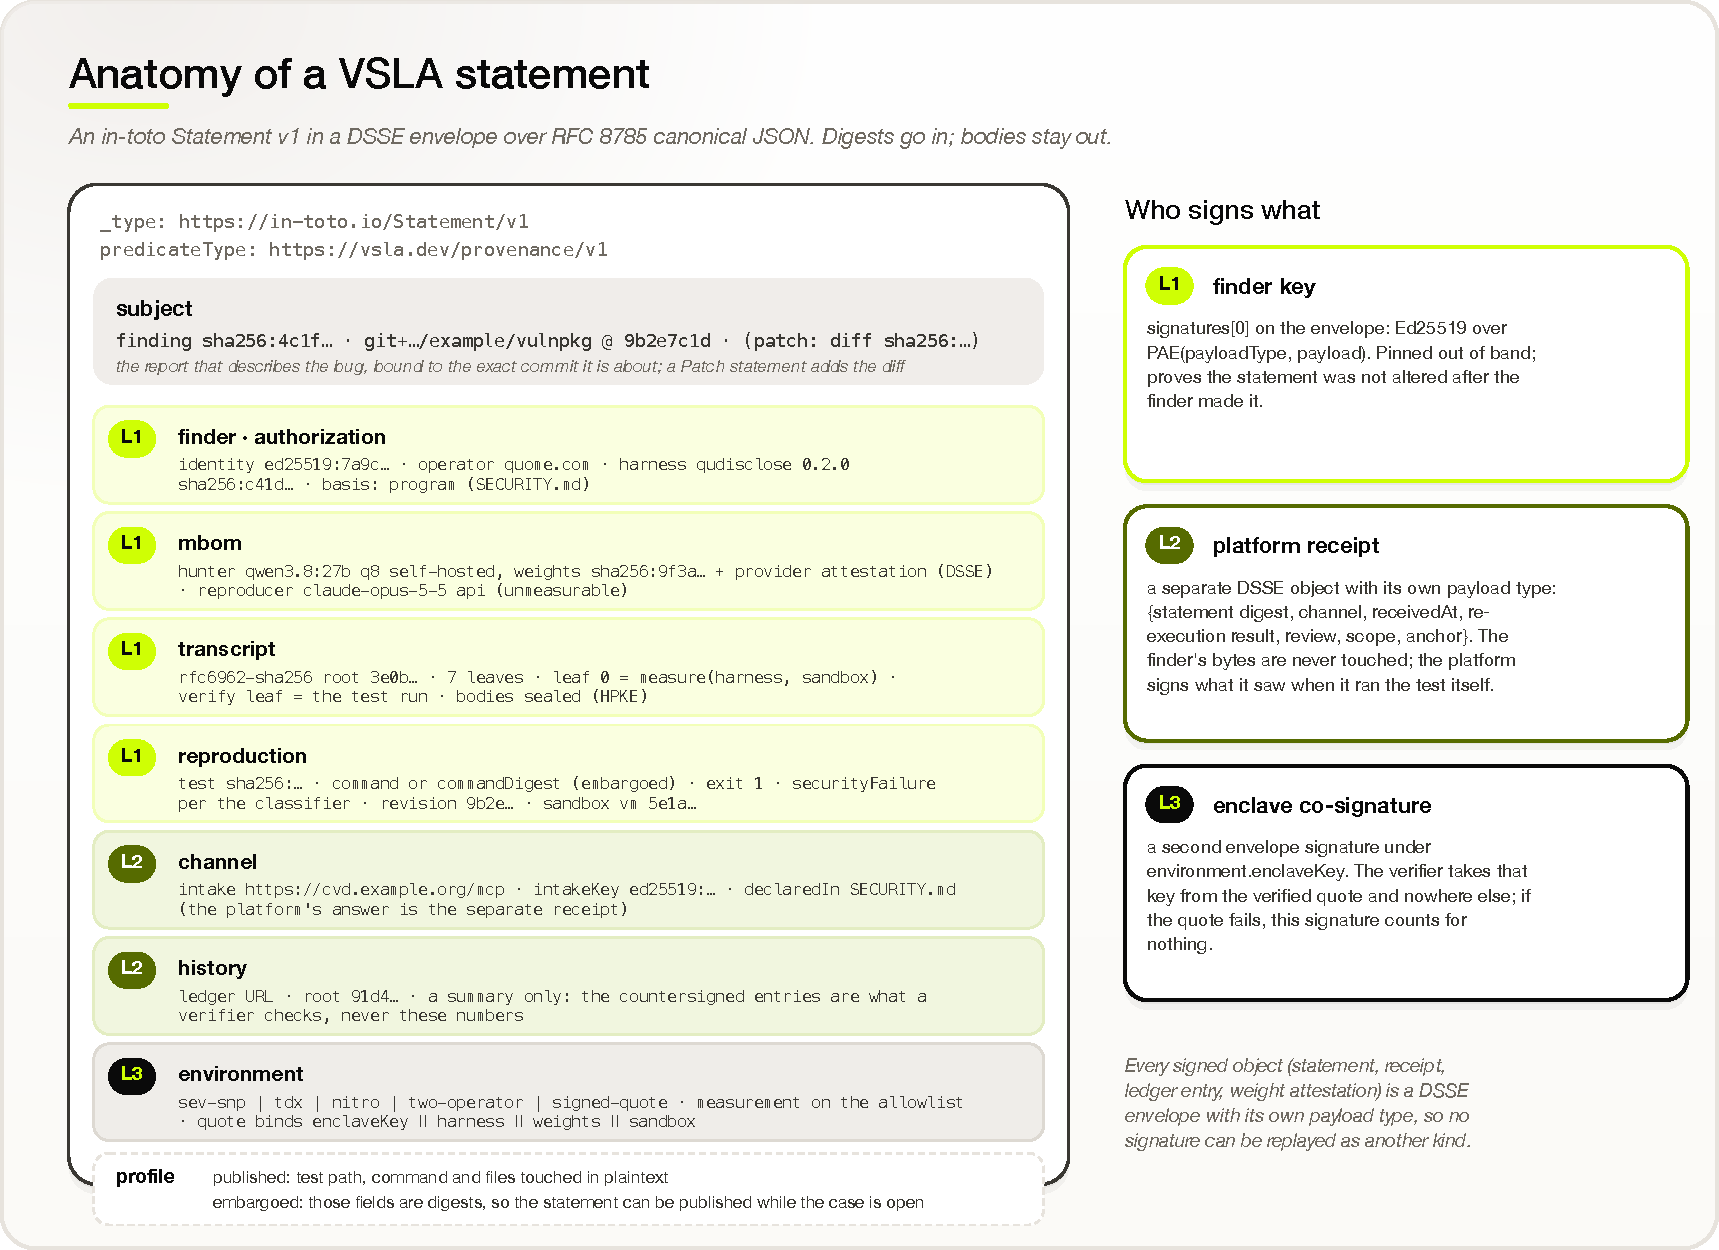
\includegraphics[width=\linewidth]{../figures/pdf/fig-attestation.pdf}
  \caption{Anatomy of a \vsla{} statement. Digests go in; bodies stay out.}
  \label{fig:attestation}
\end{figure}

A \vsla{} statement (Figure~\ref{fig:attestation}) is an in-toto Statement v1, in a DSSE envelope, whose
predicate type is \texttt{https://vsla.dev/provenance/v1}. Three further signed objects, the receipt, the
ledger entry and the weight attestation, are DSSE envelopes with their own payload types, so that no two
objects signed by one key can be confused for each other. Every canonical body is RFC 8785 JSON, and a verifier parses every
signed payload strictly: a payload that does not re-serialise to itself, or that carries a duplicate key, is
rejected, so two conforming verifiers cannot read different values from one signature. The first draft said
``sorted keys, no whitespace'' and its three implementations already disagreed on float formatting and on which
fields a ledger entry's signature covered; the second enforced nothing about the bytes it signed.

The design rule is \emph{digests go in, bodies stay out}: the statement commits to the transcript, the
proof-of-concept, the diff and the test output by digest and carries none of their text. The first draft
claimed this made a statement safe to publish during embargo, while the predicate carried the test path, the
command and the files touched in plaintext, each of which is a one-line description of the bug. A statement
now has a \emph{profile}: in the \texttt{embargoed} profile those fields are digests and the repository name
may be too; in the \texttt{published} profile they are plaintext, and the receipt's command digest lets a third
party match the two later.

\paragraph{Subject.} The digest of the report fields that describe the bug (not contact or credit) and the
git commit, which the reproduction's revision must equal. It identifies this report; the first draft also
claimed it was a deduplication key, which it is not, since two finders describe one bug differently.
A Patch-track statement adds the diff digest.

\paragraph{Authorization.} The basis on which the finder was entitled to test the code (ownership, a published
program scope, a written engagement, a safe-harbour policy) and a reference to it. \vsla{} records it and
cannot enforce it.

\paragraph{Model bill of materials.} Every model that produced or filtered content on the path to the
finding: role, provider, name, family, version, serving mode, and for self-hosted models either a digest of the
loaded weight bytes with the provider's signed attestation when one exists, or \texttt{unmeasured}. A digest of
the model's \emph{name}, which the first implementation emitted, is a false statement and is now a schema
violation. Omitting a model that took part voids the statement. When a model turns out to be bad, the MBOM
answers which disclosures it touched, exactly as an SBOM answers which builds used a vulnerable library; it is
a traceability device, not a detector.

\paragraph{Merkle-rooted transcript.} Leaves are canonical JSON of one model turn, one tool call, one
verification step, or the initial measurement of harness and sandbox. The tree is RFC 6962
(Figure~\ref{fig:merkle}); leaf 0 must be the measurement and a verification leaf must agree with the
reproduction section, both of which a verifier with the leaves checks. A tree rather than one hash lets a
finder reveal a single leaf with an inclusion proof while keeping prompts private, and makes an edited,
reordered or dropped turn visible \emph{after the root is signed}. Nothing in a tree says the finder committed
every turn it ran; completeness is a property of the recorder, and only a recorder inside a measured harness
can attest it, which is where Agent Flight Recorder~\cite{flightrecorder} also leaves it.

\begin{figure}[htbp]
  \centering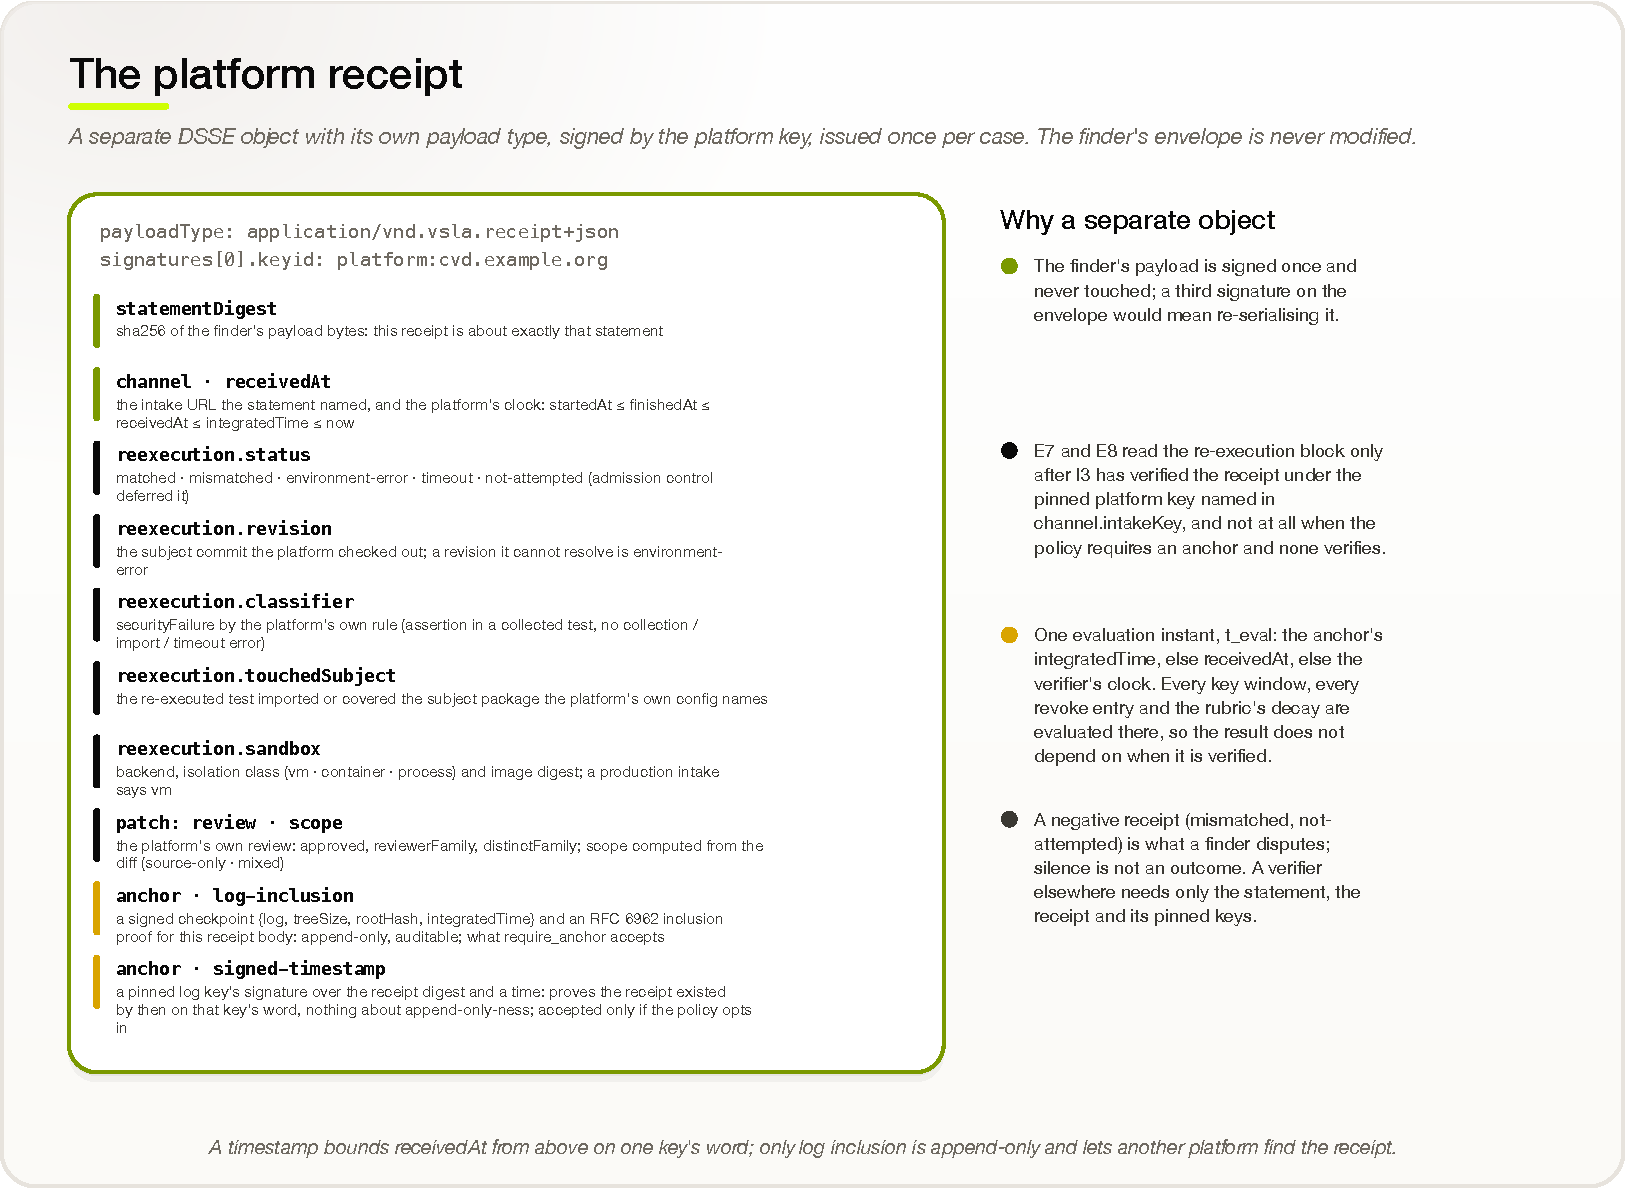
\includegraphics[width=\linewidth]{../figures/pdf/fig-receipt.pdf}
  \caption{Anatomy of the platform receipt: a separate DSSE object over the statement digest, channel, time, the platform's own re-execution result (status, revision, classifier, coverage, sandbox class), its review and scope on the Patch track, and an anchor in one of two named forms, log inclusion or signed timestamp. The finder's envelope is never modified; E7/E8 read the receipt only after I3 has verified it, and not at all when an anchor is required and absent; the anchor's time is the evaluation instant.}
  \label{fig:receipt}
\end{figure}

\begin{figure}[htbp]
  \centering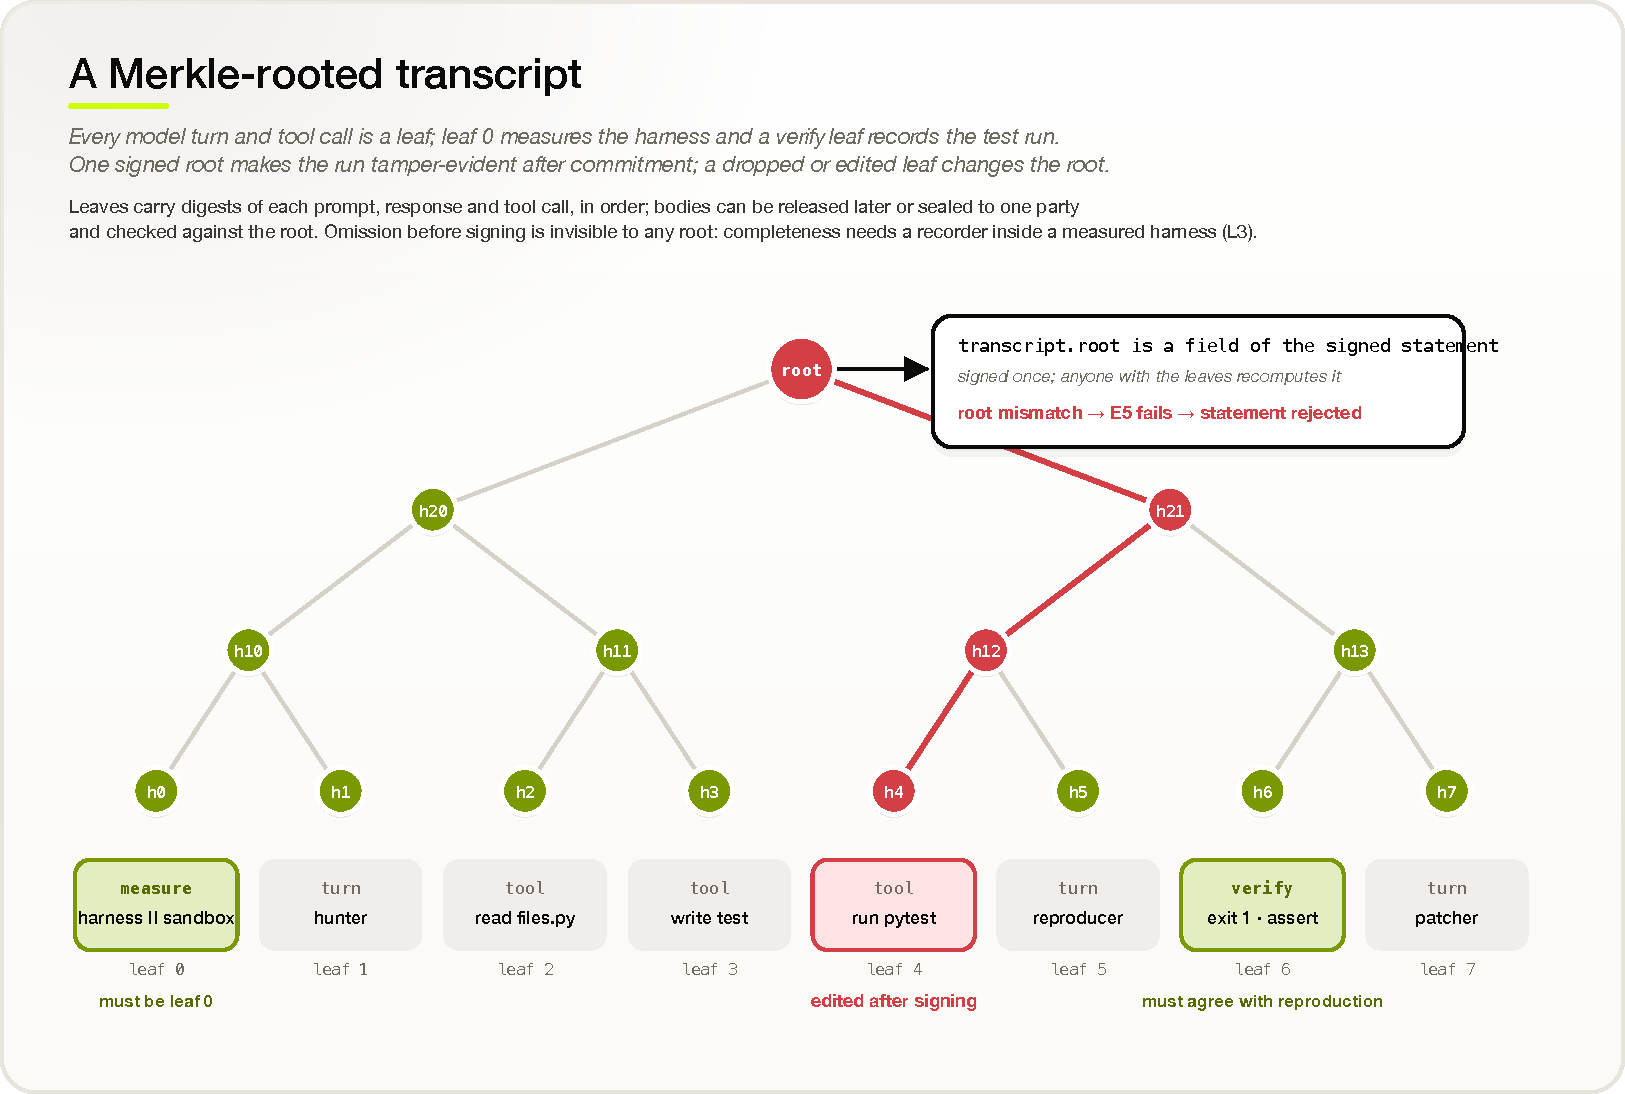
\includegraphics[width=\linewidth]{../figures/pdf/fig-merkle.pdf}
  \caption{The transcript commitment. One edited leaf changes the root; the root is signed once. Omission before signing is not visible here.}
  \label{fig:merkle}
\end{figure}

\paragraph{Reproduction.} Test digest, the command or its digest, expected and observed exit codes, the
revision executed against, the sandbox backend, isolation class and digest, the output digest, and start and
end times. The executor is \texttt{code}: a test runner produced the exit code, not a model's assertion that it
ran. The classification of the failure is by a normative rule over the runner's structured result (at least one
collected test failed by assertion; no collection, import, fixture or timeout error), not a substring search over its
output, which is what the first implementation did. The second review showed the limit of that rule: the runner
writes its report inside the process the test runs in, so a hostile test can forge it, and a test that imports the
subject and asserts false needs no forgery at all. The classifier filters honest error, and the specification now
says so; the semantic judgement is the receiver's.

\paragraph{Receipt.} The platform's countersignature is a separate DSSE object (Figure~\ref{fig:receipt}), not a
third signature on the envelope, so that the finder's payload is never modified after it is signed. The platform
signs the statement digest, the channel, the time and its own re-execution result: a status (\texttt{matched},
\texttt{mismatched}, \texttt{environment-error}, \texttt{timeout}, \texttt{not-attempted}), the revision it ran
at, its own classification, whether the test loaded the subject package and how that was decided (imported or
covered), the sandbox's backend and isolation class, and on the Patch track its own review and the scope it
computed. A receipt is issued once per case, so a finder always holds proof of receipt and a negative receipt is
what it disputes. A receipt counts only under the platform key the statement itself names in its channel, and a
verifier reads its re-execution result only after that binding has verified: the second review reached a verified
\lvl{2} with a receipt the finder had signed under its own pinned key. The first draft said the receipt settles
``who knew what, when'' without either party's cooperation; it settles it with the platform's cooperation and
honesty, and the receipt therefore may carry an \emph{anchor} in one of two named forms. \emph{Log inclusion} is a
log's signed checkpoint and an inclusion proof for the receipt body as a leaf, the shape Rekor and SCITT provide and
the one the shipped examples carry; it is what ``anchored in a transparency log'' means. A \emph{signed timestamp} is
a pinned log key's signature over the receipt digest; it proves that the receipt existed by that time on one more
key's word and nothing about append-only-ness, and the third review was right that revision 3 let it stand in for
the first. A verifier that will act on another platform's receipt runs with the anchor required, under which only
log inclusion satisfies it unless the policy opts into timestamps, and an unanchored receipt then fails and is not
read for evidence either. The anchor's time is also the \emph{evaluation instant}: every key window, every
revocation and the rubric's decay are judged at it, never at a time the checked party wrote, so the same anchored
statement verifies identically today and in a year. The anchor upper-bounds the receipt time; it cannot lower-bound
it, because a platform can hold a receipt before anchoring it, and the paper does not claim otherwise.

\paragraph{Trust ledger.} An append-only Merkle log whose leaves are the canonical bytes of countersigned
DSSE entries (Figure~\ref{fig:history}). An entry names finder, statement digest, platform, track, outcome,
claimed and verified level, a signed reason on every negative outcome, and the countersigner. Outcomes are
\texttt{accepted} (the maintainer or its authoritative agent accepted the \emph{outcome}: the fix merged, the
advisory issued; not merely ``we reproduced it''), \texttt{duplicate}, \texttt{rejected}, \texttt{false-positive},
\texttt{reproduced-unresolved}, \texttt{withdrawn}, \texttt{non-authoritative-release}, \texttt{retracted} and
\texttt{ledger-fork}, plus \texttt{successor} and \texttt{revoke} entries for key rotation. The finder's operator
owns the index: it appends entries in the order it receives them, and no countersigned entry carries a sequence
number. Revision 3 had the closing platform assign one, and the third review showed what every log engineer knows:
two honest platforms closing cases for one finder both assign the same number, and the finder forks through no fault
of its own. A finder keeps one ledger per track and every entry names the finder's key or a predecessor in its
successor chain; a verifier drops entries that name another key or another track, because the second review borrowed
another finder's published ledger and spent Finding history on the Patch track; and the rubric's window is the last
fifty entries by countersigned time, which the finder cannot choose, so the reordering that moved a score from $0.37$
to $0.93$ in the second review now moves nothing. The finder's operator keeps the canonical copy and every platform
that wrote to it keeps a mirror; a platform stores the root and count of the ledger it was \emph{shown}, checks on
the next submission that the prefix is unchanged and that every entry the platform itself countersigned is
\emph{included}, at any position, and records a fork otherwise (Figure~\ref{fig:consistency}). Inclusion rather than
position is what lets concurrent closes at several platforms coexist; omission of a platform's rejection is now
unambiguous and disqualifying. This detects a split view only between platforms that compare notes. The first draft said ``a finder cannot present a trimmed history''; it
can, to a platform that has never seen it, and the specification now says so and names a shared transparency
log as the remedy. Until then a ledger is evidence about the finder's history \emph{with the countersigners the
reader has pinned}, which is also exactly what the rubric computes.

\begin{figure}[htbp]
  \centering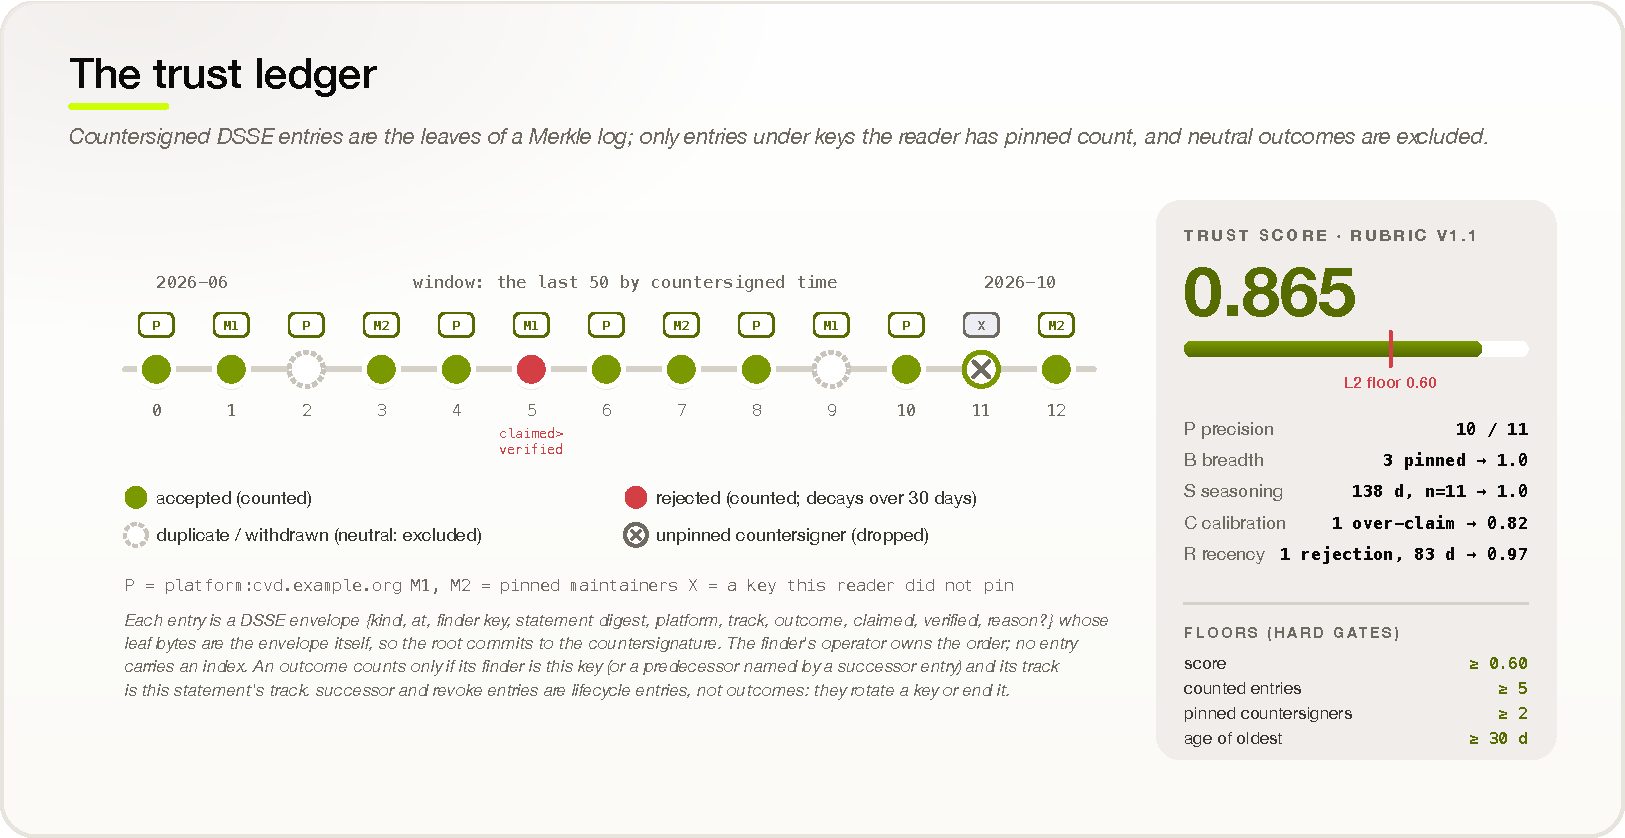
\includegraphics[width=\linewidth]{../figures/pdf/fig-history.pdf}
  \caption{The \lvl{2} ledger: countersigned outcomes become a score, and the score has a floor. Only entries countersigned by keys the reader has pinned, naming this finder's key and this track, count.}
  \label{fig:history}
\end{figure}

\begin{figure}[htbp]
  \centering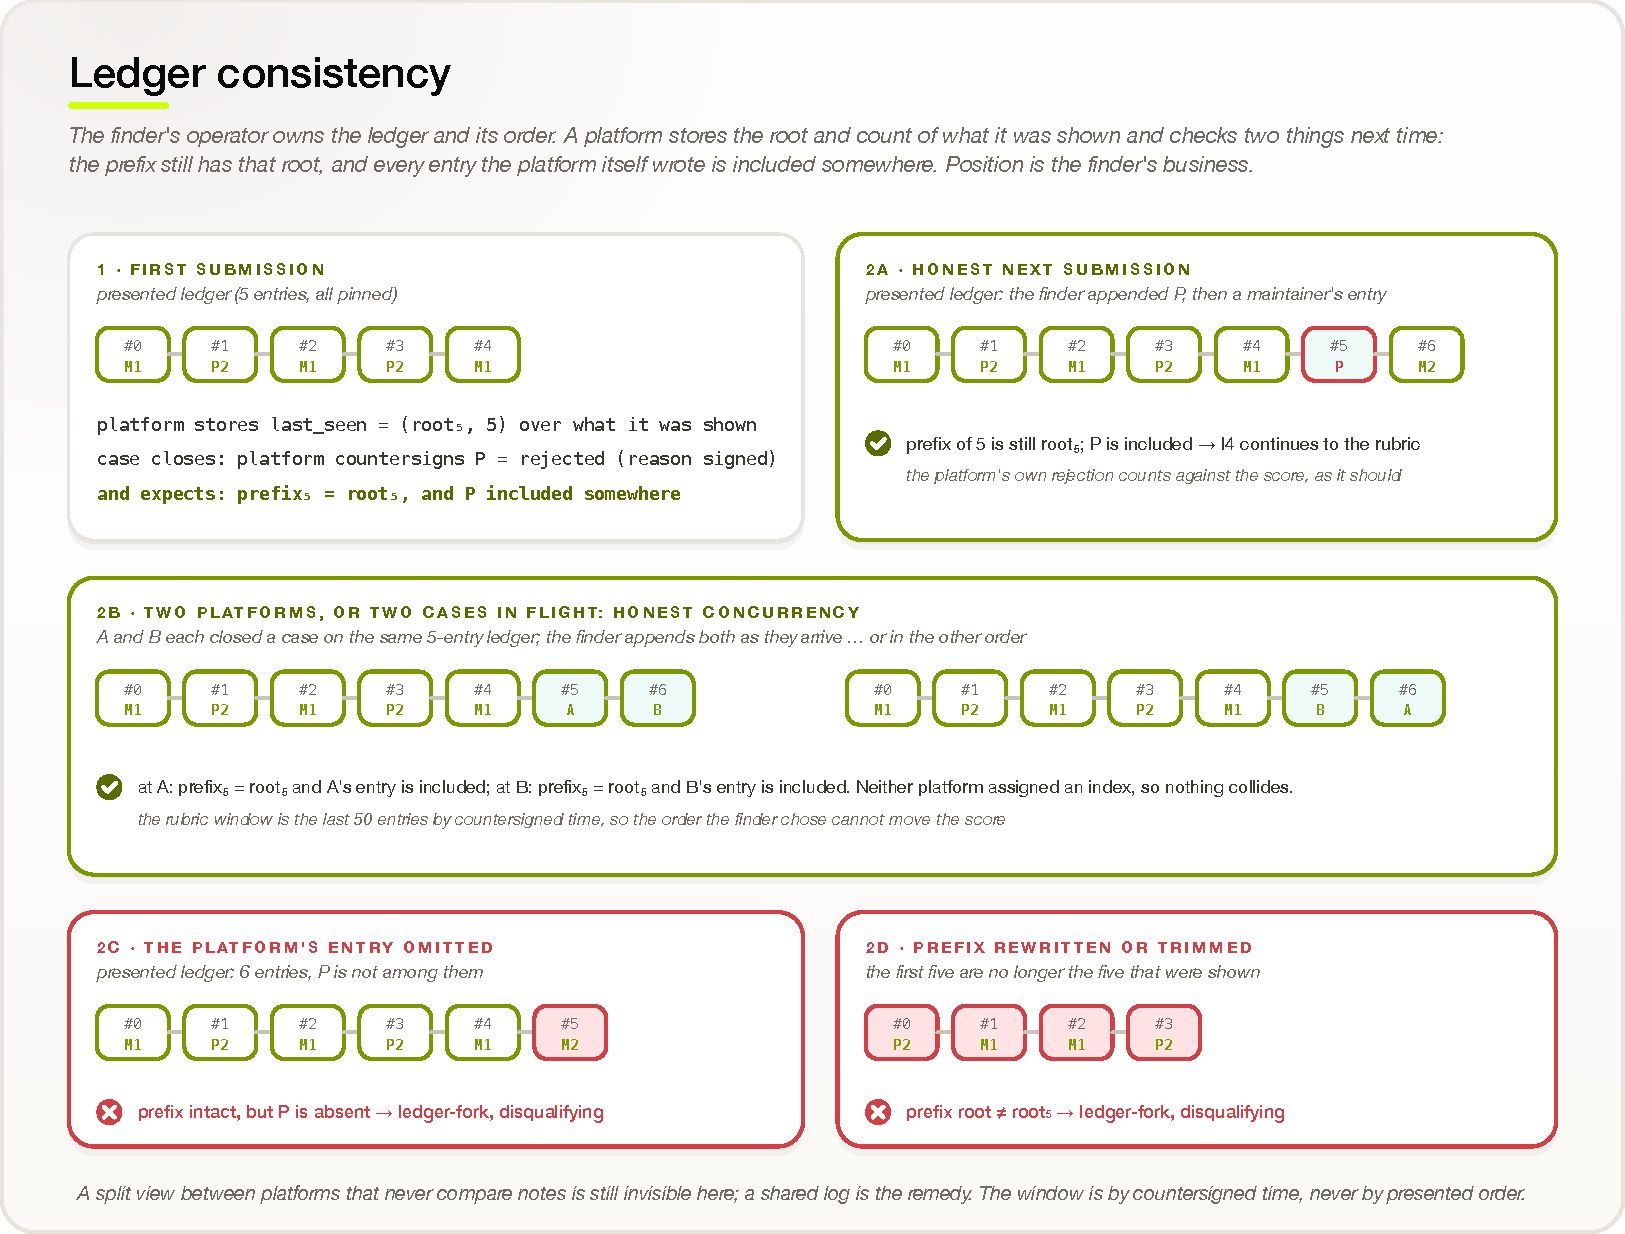
\includegraphics[width=\linewidth]{../figures/pdf/fig-consistency.pdf}
  \caption{Ledger consistency. The platform stores the root and count of the ledger it was shown and the entries it countersigned; the next ledger must keep that prefix and include those entries at any position, so concurrent closes at several platforms coexist, while a rewritten prefix or an omitted entry is a ledger-fork. Split views across platforms that never compare notes need a shared log.}
  \label{fig:consistency}
\end{figure}

\paragraph{Environment.} Type (\texttt{sev-snp}, \texttt{tdx}, \texttt{nitro}, \texttt{two-operator}, or the
reference \texttt{signed-quote}), the measurement, what it covers, the quote, the root of trust, and the enclave
key. The quote binds four things: the enclave key, the harness digest, every weight digest and the sandbox
digest; a verifier derives those from the statement and asks the adapter for that environment type whether the
quote binds exactly them. The first draft had the verifier \emph{pin} the enclave key in its keyring, which
inverts attestation; the key now comes from the verified quote and nowhere else. The specification also says,
per environment type, where the bindings live, because the launch digest of a confidential VM covers the guest
image and not the tens of gigabytes of weights loaded after boot: for SEV-SNP and TDX the bindings go through
\texttt{REPORT\_DATA}, which carries the digest of the same canonical binding body the reference adapter signs,
and a measured integrity root, and a reference measurement without a reproducible guest image means only ``some
VM ran under SEV-SNP''. A two-operator quote must be co-signed by two distinct pinned roots; one root listed twice
is one operator, which is what the second review's probe presented. The reference adapter proves only that a
pinned root key signed the bindings, is never allowlisted in production, and hardware adapters are not
implemented.

\paragraph{Keys.} A finder key is rotated with a \texttt{successor} entry signed by the old and the new key, and a
verifier follows the chain backwards from the pinned current key so that outcomes earned under the old key count
for the new one; it is revoked with a \texttt{revoke} entry signed by the operator, which fails the statement when
the revocation is not after the evaluation instant. Pinned keys carry validity windows, judged at the same instant.
``Dated after a revocation'' means dated by the anchor or the verifier, never by the key holder: the third review
showed a revoked key verifying a statement whose finder-written finish time predated the revocation. The first draft
had no key lifecycle at all, which for a reputation system means a stolen key is a stolen reputation; the third draft
specified one and implemented none of it, which the third review called out.

\section{Verification and the trust rubric}
\label{sec:verification}

\begin{figure}[htbp]
  \centering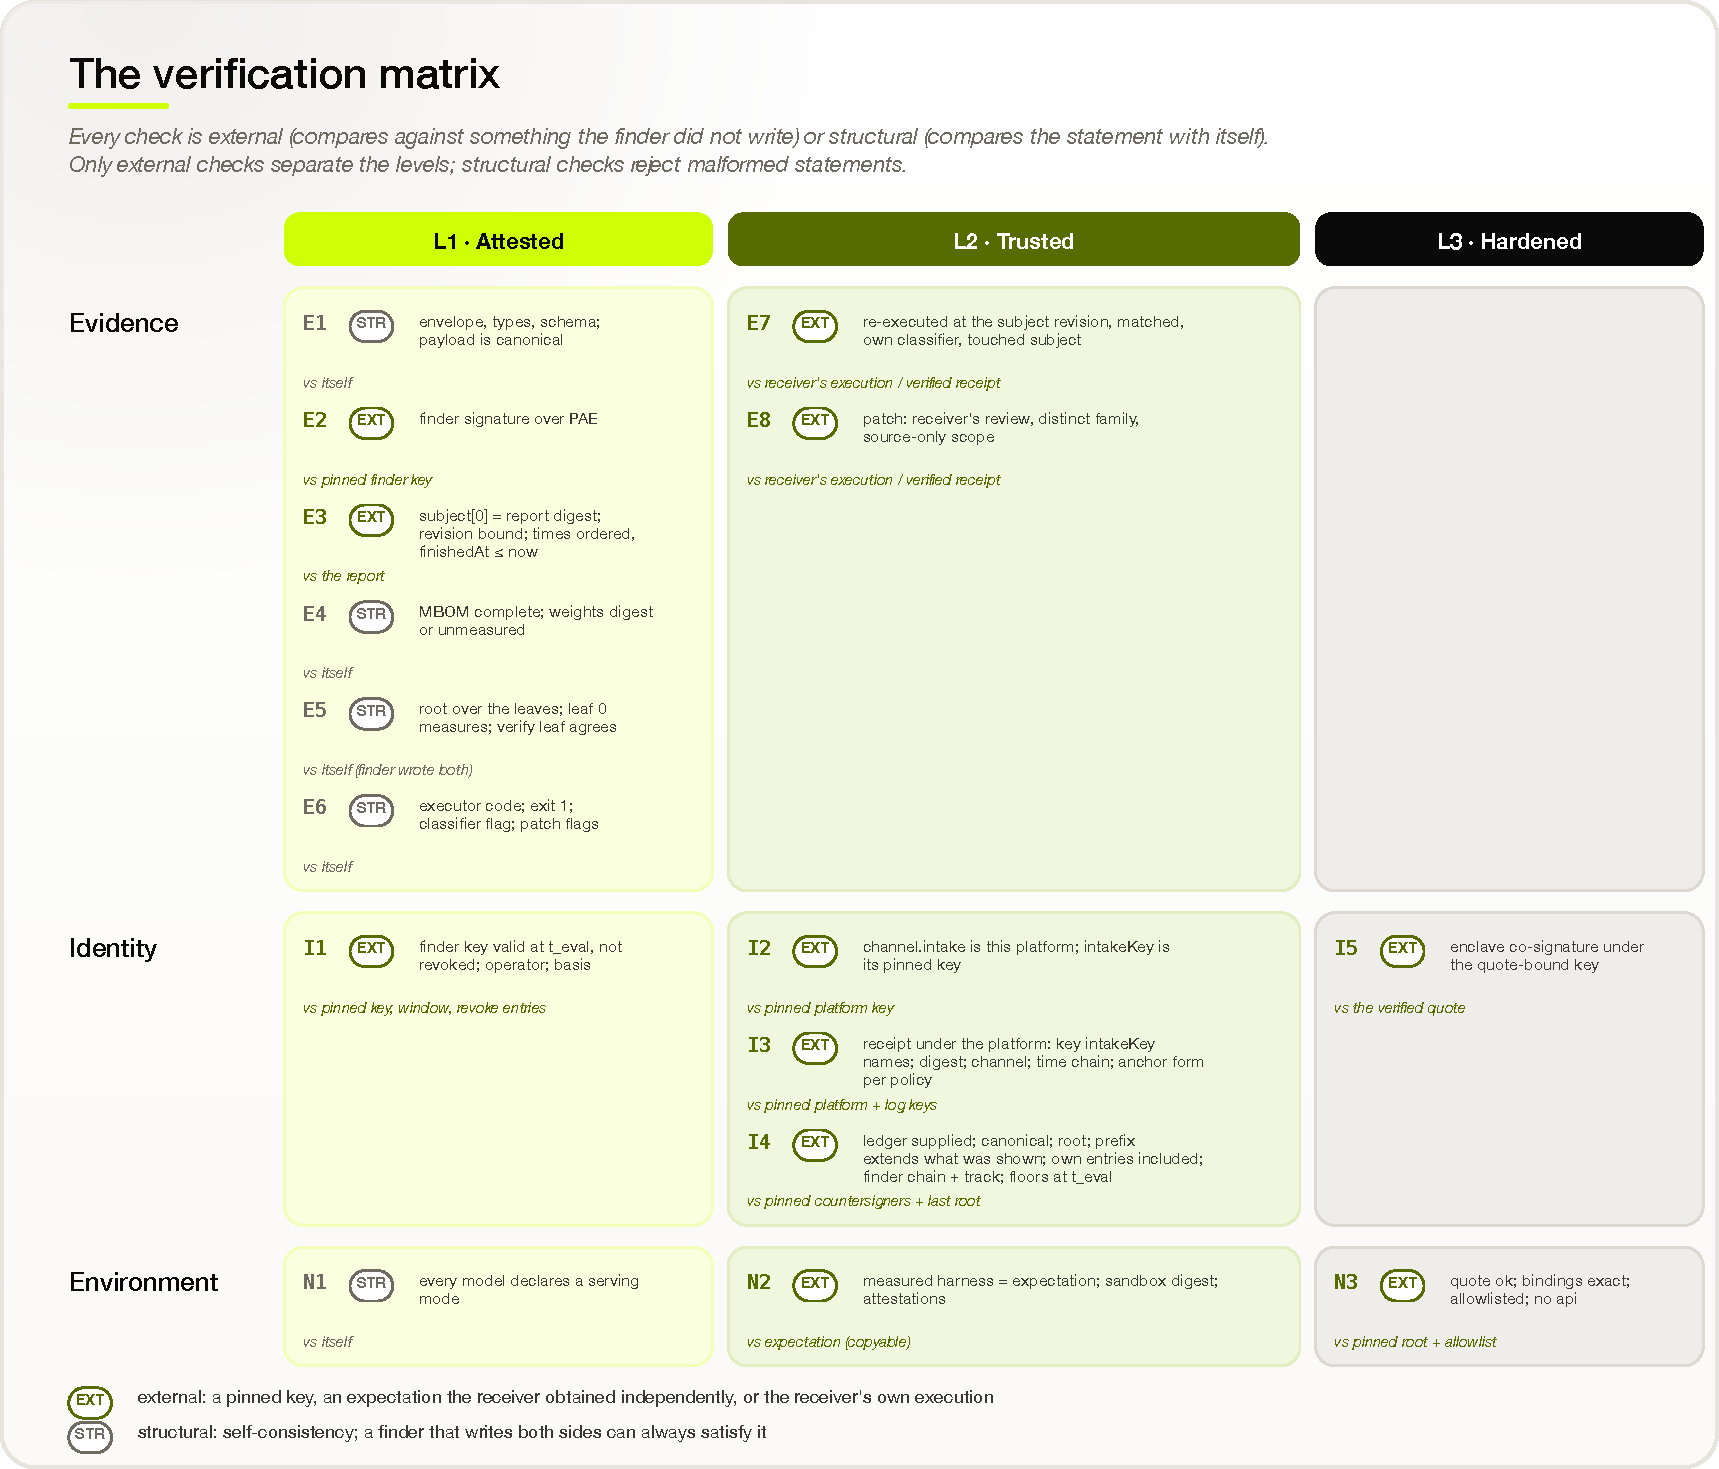
\includegraphics[width=\linewidth]{../figures/pdf/fig-checks.pdf}
  \caption{The verification matrix. Every check by pillar and level, marked external (compares against a pinned key, an expectation, or the receiver's own execution) or structural (compares the statement with itself), with what it compares against. Only external checks separate the levels.}
  \label{fig:checks}
\end{figure}

\begin{figure}[htbp]
  \centering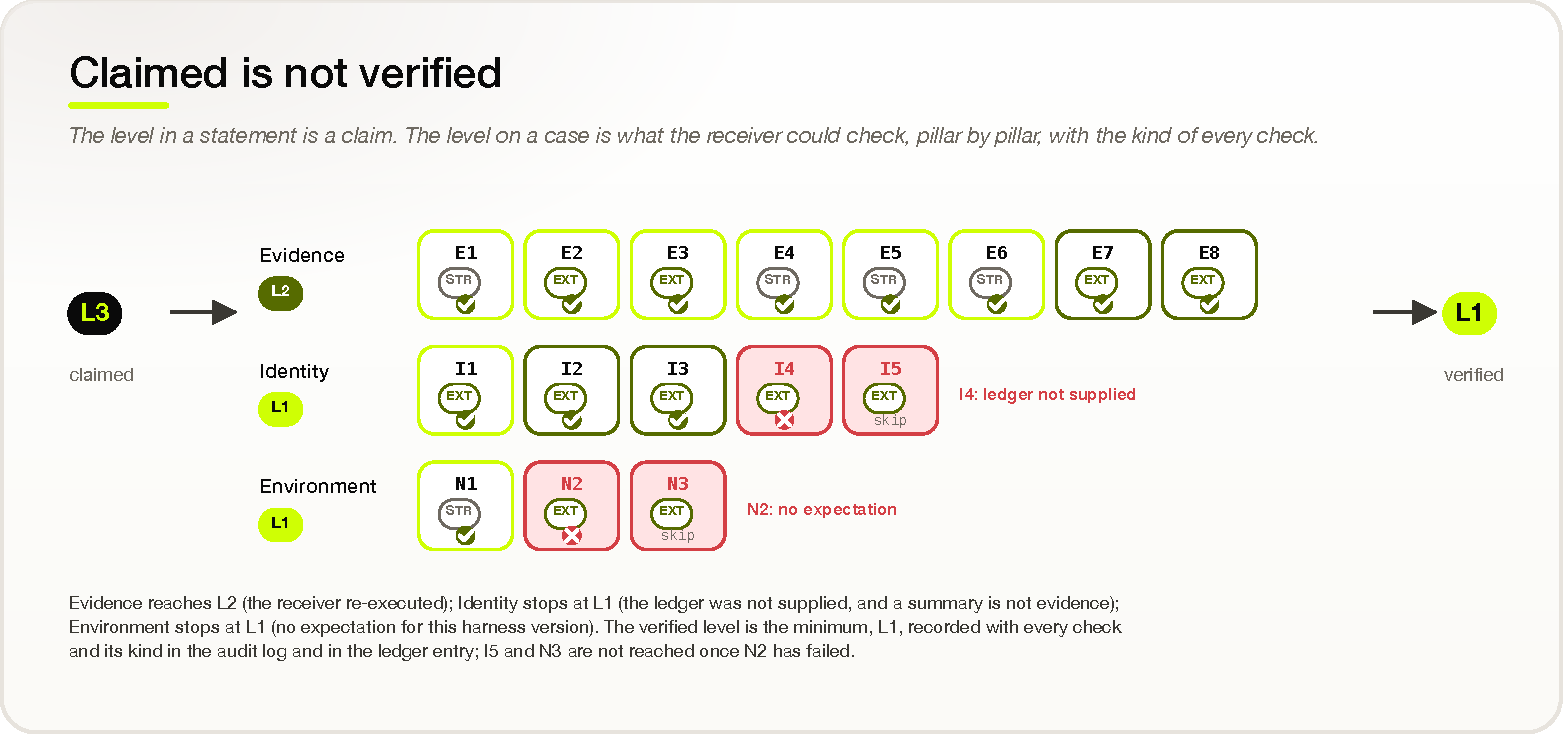
\includegraphics[width=0.92\linewidth]{../figures/pdf/fig-verified.pdf}
  \caption{A claimed \lvl{3} verified as \lvl{1}: the weakest pillar sets the level, and every check is recorded with whether it was external or structural.}
  \label{fig:verified}
\end{figure}

\begin{figure}[htbp]
  \centering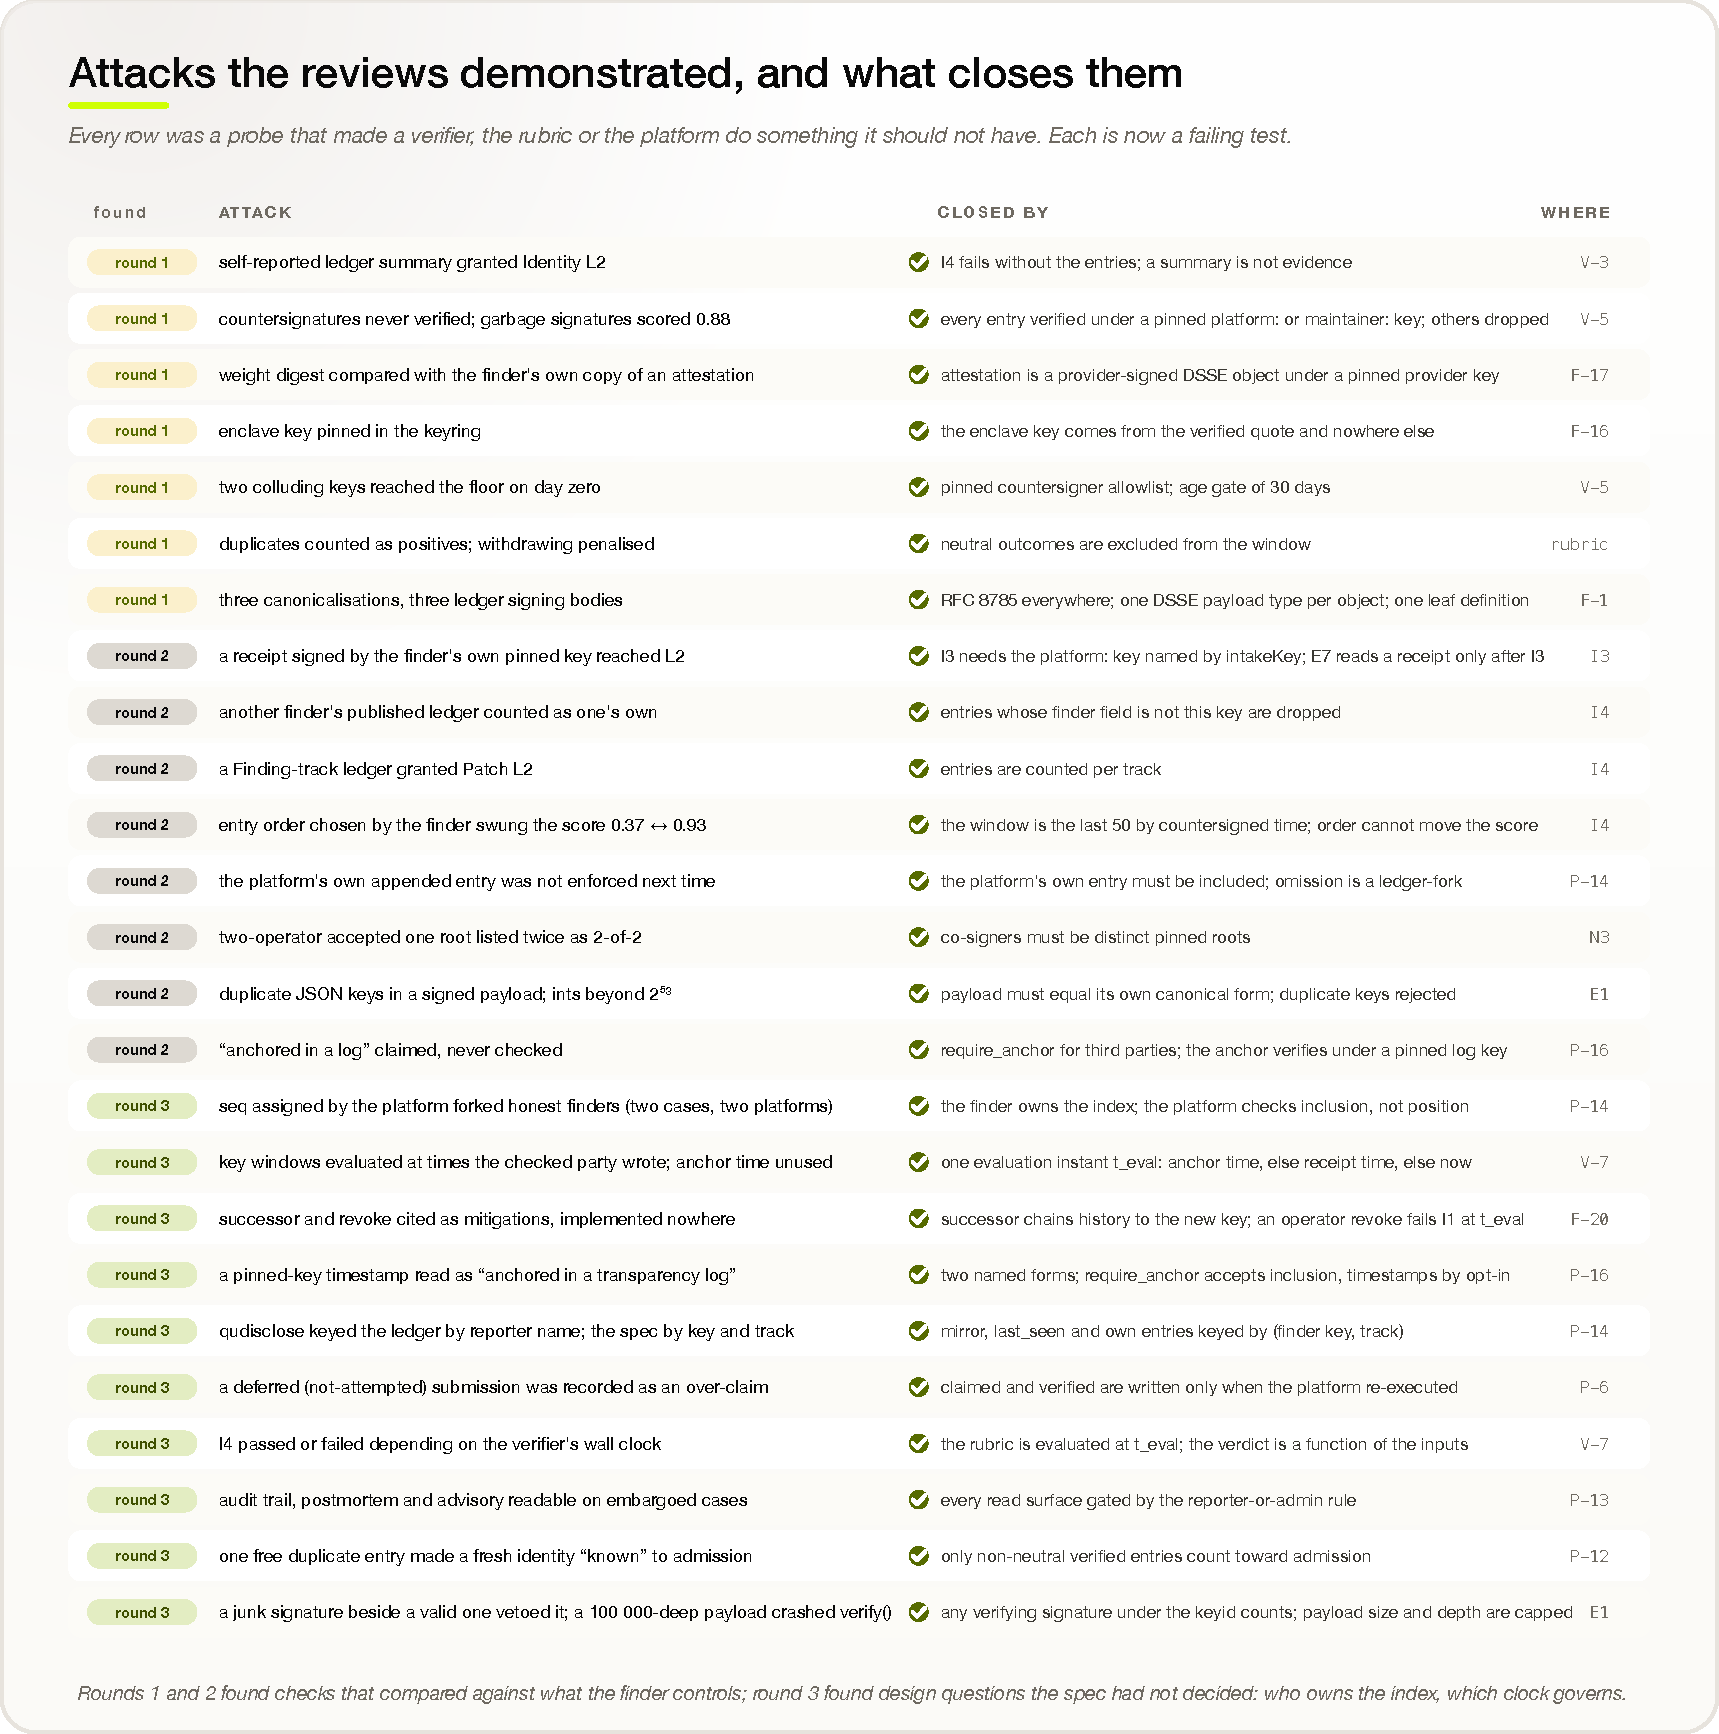
\includegraphics[width=\linewidth]{../figures/pdf/fig-attacks.pdf}
  \caption{Attacks demonstrated by five reviews over three rounds against the verifier, the rubric and the ledger, and the rule or check that now closes each; every row is a failing test in the reference suite.}
  \label{fig:attacks}
\end{figure}

A statement carries a \emph{claimed} level. A receiver computes a \emph{verified} level, which is what it
records, shows and feeds into policy. The procedure runs the checks of each pillar in order (E1--E8, I1--I5,
N1--N3; Figure~\ref{fig:checks}) against pinned keys and \emph{expectations} obtained out of band: harness digests
per name and version, and for \lvl{3} an allowlist of acceptable (environment type, measurement, harness)
triples. A pillar's level is the highest whose checks all passed, and the verified level is the minimum across
pillars and the claim (Figure~\ref{fig:verified}). Six properties follow. A missing or malformed input fails
the check that needs it rather than raising an error, so a coordinator who holds the statement but not the code
lands at Evidence \lvl{1}, and a verifier without expectations lands at Environment \lvl{1}, which are the honest
answers. Every time-dependent check is judged at one evaluation instant, the anchor's time when there is one, the
receipt's otherwise, the verifier's clock failing both, so a verification is a function of its inputs; the third
draft judged each key at a time its holder had written and recomputed the rubric at the verifier's wall clock, so
the same statement could pass today and fail next month. A self-reported value never substitutes for an input: the first draft's reference verifier granted
Identity \lvl{2} on the finder's own history summary when no ledger was supplied, and a ledger whose every
signature was replaced by garbage scored the same as the real one. A countersignature counts only under the key
the statement binds itself to: the second draft accepted a receipt under any pinned key, including the finder's
own, and read its re-execution result before checking who signed it. The verifier with the code must re-execute
the reproduction itself at the subject revision; a platform's receipt is evidence for a third party, not a
substitute for the verifier's own run. And both the claim and every check, with its kind, go into the platform's
audit log and into the ledger entry. Every attack the five reviews demonstrated is a failing test in the
reference suite (Figure~\ref{fig:attacks}); the pattern the first two rounds share is a check that compares against
something the finder controls, or does not compare at all, which is why the matrix names, for every check, what it
compares against; the third round's pattern is a design question the specification had not decided, which is why
the specification now says who owns the ledger's index and which clock governs validity.

\paragraph{Trust score.} Within a level, the ledger yields a score that platforms use to rank, route and
rate-limit and that sets the \lvl{2} floor. After dropping entries whose countersignature does not verify under
a pinned key, and excluding \emph{neutral} outcomes (duplicate, withdrawn, reproduced-unresolved) from the
window entirely, over the last $W=50$ counted entries with $n$ entries,
$a$ accepted (not vouched), $m$ distinct pinned countersigning operators, $o$ over-claims, $age$ days of history and
$r_i$ the age of each rejection:
\begin{align*}
P &= \tfrac{a}{n}, \qquad B = \min(1, \tfrac{m}{3}), \qquad S = \min(1,\tfrac{age}{90})\cdot\min(1,\tfrac{n}{10}),\\
C &= \max(0, 1-\tfrac{2o}{n}), \qquad R = 1 - \tfrac{1}{2}\min\!\Big(1, \textstyle\sum_i e^{-r_i/30}\Big),\\
\text{score} &= 0 \text{ if any entry is disqualifying or } o/n \ge \tfrac12, \text{ else } P\,(0.5 + 0.2B + 0.2S + 0.1C)\,R.
\end{align*}
The default floor for \lvl{2} is $0.60$ with at least five counted entries from at least two distinct pinned
countersigners and a ledger at least 30 days old; the age is a gate, not a term. Every change from the first
rubric closes a specific attack a reviewer demonstrated. Duplicates counted as positives, so a finder could
farm them from public cases; they are now neutral. Withdrawing was penalised, which punishes the behaviour you
want. Recency looked only at the most recent rejection, so ten rejections last month scored as one; it now sums
them with decay. Calibration carried a tenth of the weight, so over-claiming \lvl{3} on every statement cost
$0.1$; it is now twice as steep and disqualifying at half the window. And two colluding keys with five
accepted entries scored $0.733$ on day zero, above the floor; the age gate and the countersigner allowlist
close that, and the specification says plainly that two countersigners is a floor on distinct pinned operators
(two keys of one operator are one countersigner), not on independence. A new finder has no ledger and therefore no \lvl{2}; that is intended. It discloses at \lvl{1} to
platforms that accept \lvl{1} into a slower lane, collects countersigned outcomes, and crosses the floor the way
a contributor earns commit rights. An honest finder that discloses to a single platform has one countersigner
and cannot reach \lvl{2} there until a maintainer countersigns directly or vouches; the specification accepts
that cost rather than count a platform's self-countersigned entries twice.

\section{Implementation in qudisclose}
\label{sec:impl}

\begin{figure}[htbp]
  \centering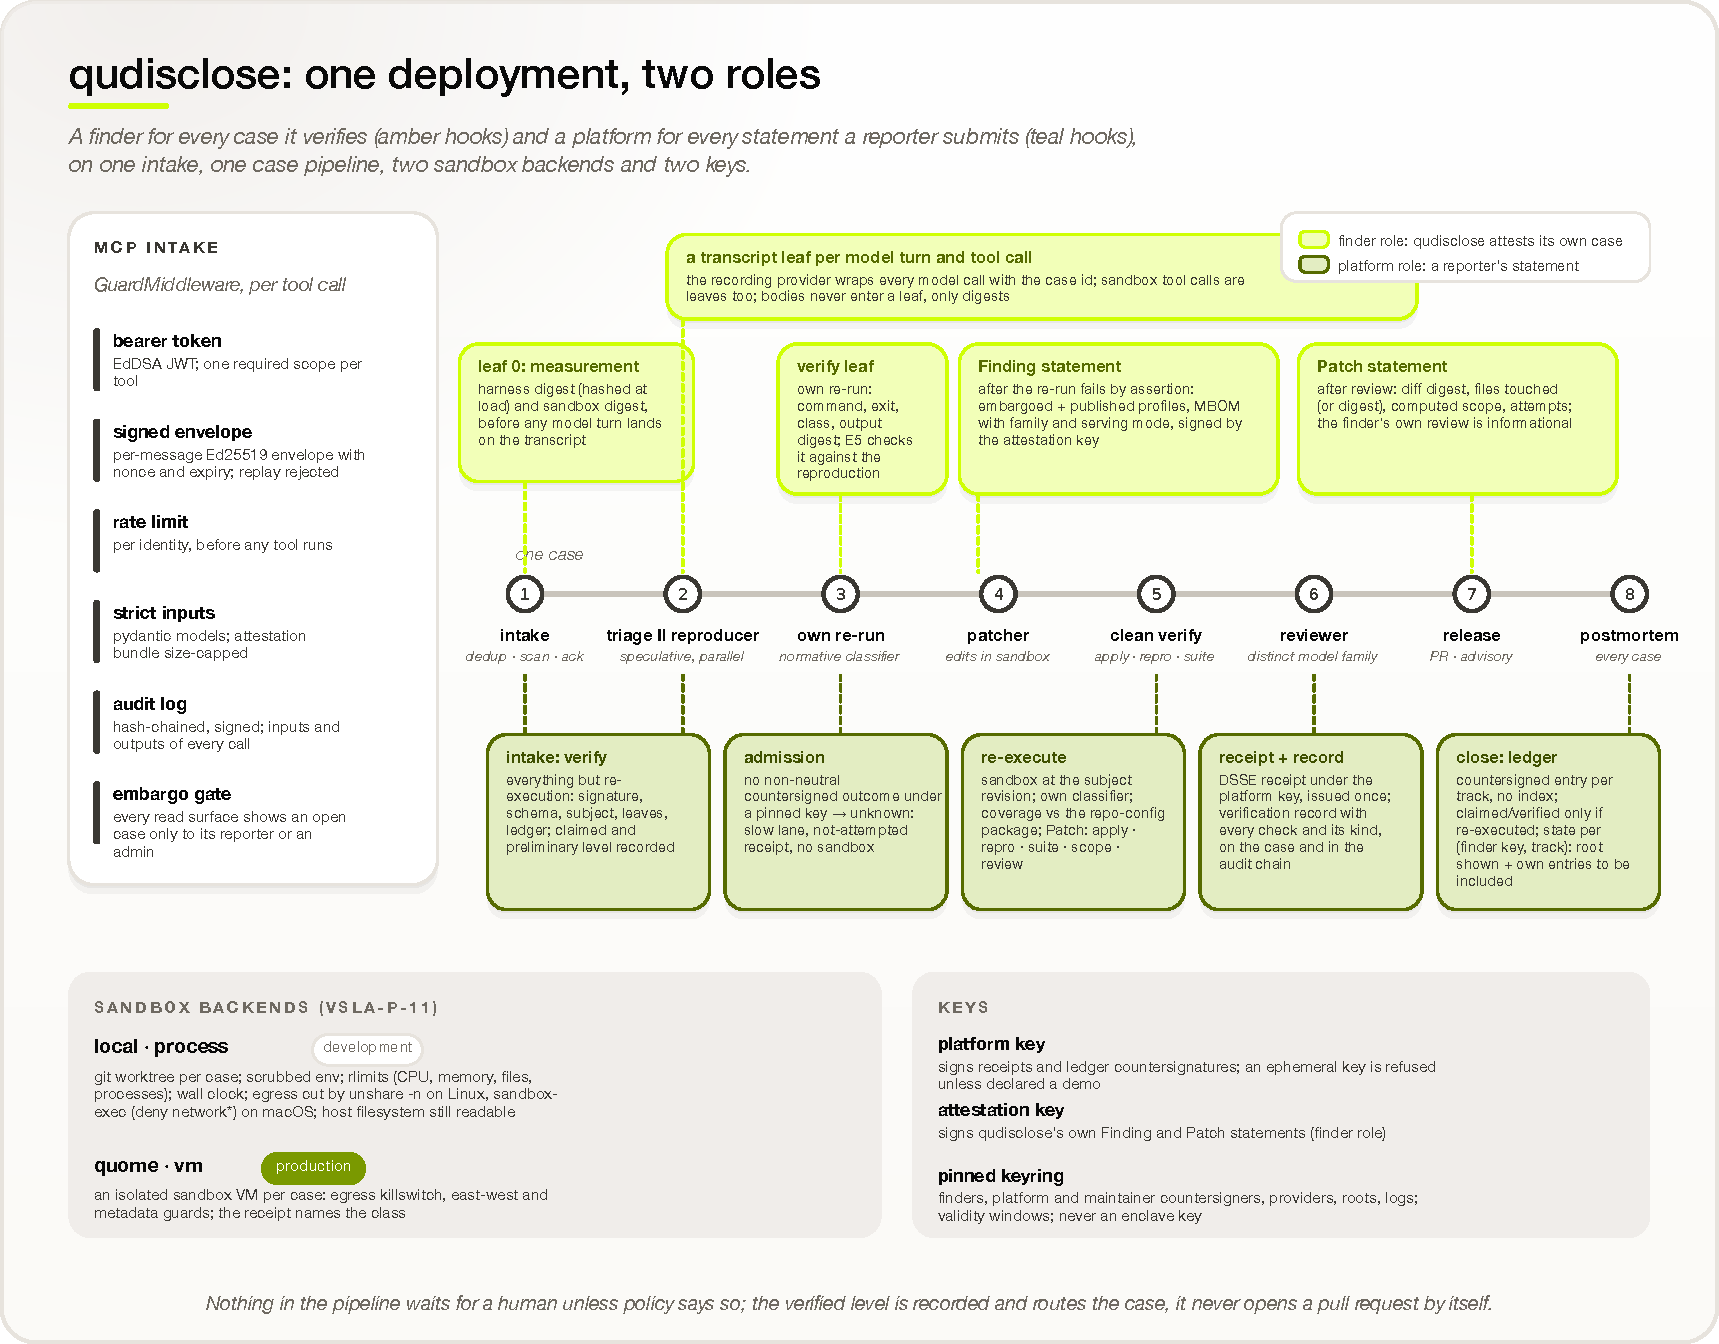
\includegraphics[width=\linewidth]{../figures/pdf/fig-qudisclose.pdf}
  \caption{qudisclose in both roles. One intake (scoped bearer tokens, signed per-message envelopes, a hash-chained audit log, every read surface gated until the case is public) feeds one case pipeline. Above the timeline, the finder-role hooks that produce qudisclose's own statements: the measured first leaf, a transcript leaf per model turn and tool call, the verify leaf at the orchestrator's own re-run, and the Finding and Patch statements signed by the attestation key. Below it, the platform-role hooks for a submitted statement: verification at intake, admission control, re-execution at the subject revision with the platform's own classifier and coverage check, the receipt issued once under the platform key, and the countersigned per-track ledger entry at close, with consistency state kept per finder key and track. Only the VM sandbox backend is production-grade.}
  \label{fig:qudisclose}
\end{figure}

qudisclose~\cite{qudisclose} is a machine-to-machine disclosure platform: an MCP intake with bearer tokens
and Ed25519-signed envelopes, a team of agents (triage, reproducer, patcher, reviewer, release, postmortem),
code-side verification in clean worktrees, a hash-chained and signed audit log, and an always-on hunter that
runs on self-hosted models (Figure~\ref{fig:qudisclose}). The \vsla{} layer, as revised after review, adds:

\begin{itemize}
  \item \textbf{Transcript capture.} A recording provider wraps every model call with the case id and appends a leaf to the case's transcript; sandbox tool calls and the orchestrator's own run of the reproduction are leaves too. Leaf 0 is the measured harness and sandbox digest; a verification leaf records the test run.
  \item \textbf{Statements on both tracks.} When the orchestrator has verified the reproduction it emits a Finding statement in the embargoed profile; when a patch has passed reproduction, suite and review it emits a Patch statement with the computed scope. The MBOM names each model's family and serving mode; a self-hosted model carries a digest of its weight file when the operator configured one and \texttt{unmeasured} otherwise. Statements are signed by the deployment's attestation identity, stored as case artifacts, and served over MCP in the embargoed profile until the case is public.
  \item \textbf{Receipts and verification at intake.} A submission may carry a statement. The intake verifies it against its own expectations (its harness digest for the running version), re-executes the reproduction at the subject revision in a clean sandbox, classifies the result from the runner's structured output (written to a per-run random path and cross-checked against the runner's own summary and exit code; it defends against honest error, not a hostile test, as Section~\ref{sec:provenance} says), checks that the test imported or covered the package the platform's repository configuration names (never a name the report supplies) and records which, and for a Patch statement applies the diff, runs the reproduction and the suite, computes the scope from the diff's git headers as well as its hunks (so renames, mode changes, binary patches and submodule edits are \texttt{mixed}), and runs its own reviewer on a different model family when one is configured (recording \texttt{distinctFamily: false} honestly when it is not). It signs a DSSE receipt once per case, with \texttt{not-attempted} when admission control defers an identity that presents no verifiable ledger, which is the default, and records claimed and verified levels on the case and in the audit chain. The verified level is recorded; it does not by itself open a pull request, which the first draft claimed and the code never did.
  \item \textbf{Ledger.} Countersigned DSSE entries per reporter identity and per track, appended when a case closes, with \texttt{accepted} reserved for cases that were published and \texttt{reproduced-unresolved} for the rest, an auditable reason on every negative outcome, never a \texttt{false-positive} over a receipt whose re-execution of the finder's own test matched, claimed and verified levels recorded only when the platform re-executed, and, per finder key and track, the root and count of the ledger the platform was shown plus the entries it countersigned, so that a history that rewrites the prefix or omits one of them is recorded as a fork while concurrent closes elsewhere are not. The rubric is computed on demand and the floors, admission limits, isolation class and pinned countersigners are published in the policy resource.
  \item \textbf{Scoping.} The ledger endpoint returns only the caller's own entries; every read surface, including the audit trail, postmortem and advisory, withholds an embargoed case from anyone but its reporter and the maintainer (the third review found three of seven ungated); the embargoed statement names the repository by digest; admission counts only non-neutral countersigned outcomes, so a free \texttt{duplicate} makes no identity known; the hunter refuses to start without an explicit allowlist of authorised targets.
  \item \textbf{Environment adapters.} The Environment pillar is a pluggable attestor. The reference adapter is the signed-quote form; SEV-SNP and TDX quote verification are vendor-library integrations and are explicitly \emph{not} claimed as implemented. The deployment's patch agents call a model through an API, so its own statements cannot verify above \lvl{2} on the Environment pillar.
\end{itemize}

The default local sandbox is process-level isolation and is a development convenience: on macOS, where the
authors' hunter runs, it denies network through \texttt{sandbox-exec} and nothing else, and the receipt says so; a
production intake must use the VM-backed sandbox, and the receipt says which was used, so a reader of any receipt
can tell a pilot-grade re-execution from a development one. The \vsla{} repository ships a reference
verifier and signed examples on both tracks at every level, which the implementation's tests cross-check for
byte compatibility. Not every requirement id has a test that cites it; the ones that do are listed in the
specification.

\section{Pilots}
\label{sec:pilots}

Nothing in this paper has been measured yet. The framework, the predicate, the verifier and the implementation
exist; the evidence that any of it changes a maintainer's behaviour does not. The hypothesis we intend to test is
narrow: \emph{a machine-generated patch that arrives with a verified \vsla{} Patch \lvl{2} statement is accepted
more often, and no less safely, than an otherwise identical unattested one}. We are in discussions with pilot
partners now, and we keep the design broad here rather than commit partners or dates to print before they
have agreed to them.

\paragraph{What a pilot measures.} ``Merged faster'' on its own is the wrong headline: time-to-merge rewards
exactly the behaviour that let xz-utils through and that bounty fraudsters optimise for, and a pilot that
reports only speed and acceptance will be read, correctly, as ``we made maintainers review less''. The primary
metrics are therefore paired: acceptance rate and time-to-merge against the partner's existing baseline for
machine-generated patches, \emph{and} post-merge revert and regression rate, defects found in attested patches
by later review, and false-acceptance rate on a seeded adversarial set (self-fulfilling tests, injected
proofs-of-concept, scope-creeping diffs). Secondary metrics are maintainer minutes per case \emph{per level},
false-positive rate per finder identity, how fast a new identity climbs from \lvl{1} to \lvl{2}, and
maintainer-reported confidence. A pilot that cannot report the baseline is not a pilot, and a design that
blinds maintainers to the arm needs a third arm in which the same pipeline runs but the statement is withheld,
so the comparison measures the badge and not the pipeline behind it.

\paragraph{Two settings.} In a \emph{partner-hosted} pilot, an established project with a mature release
process and an existing stream of machine patches pins its intake and policy as the authoritative channel and
receives attested patches on already-triaged bugs. In a \emph{staging} pilot, the hunter runs against a
\emph{private} fork of a package ecosystem on self-hosted weights, attests every reproducible finding, and
patches the fork. The first draft had the staging pilot notify upstream after a fixed window; that is the
inverse of coordinated disclosure, and the guardrail it stated (``never earlier'') had the direction wrong.
Each upstream is notified through its declared channel at discovery; the fork stays private; nothing about a
finding is published until upstream has shipped or its own deadline has passed; and there is no public
``hardened fork'', which would be a non-authoritative release of fixes by the paper's own T6.

\paragraph{Guardrails.} Both settings run only on code the operator owns or is authorised to test, with the
authorisation basis in every statement and an explicit allowlist in the hunter's configuration. Both run the
intake's re-execution with VM isolation on the operator's own hardware; the receipts name the isolation class, and
a pilot whose receipts say \texttt{process} is not the pilot described here. The whole
pipeline, not only the hunter, runs on self-hosted weights in the pilots, so that no partner source reaches a
third-party model provider; the first draft claimed this while the default configuration sent source to an
API. Results, including null results, will be published with rubric inputs in aggregate; per-case ledger
entries name partner projects and timings and will not be published. Running a hunter against third-party
code, even on a private fork, is lawful only under authorisation or safe harbour, and the paper says so
rather than leave it implied.

\section{Discussion}
\label{sec:discussion}

\paragraph{Trust the badge.} The intended effect of a level, ``a maintainer can sleep'', is also its failure
mode. Every signal that reduces review attention is eventually targeted, and the response of mature programs
to AI-era reports has been more verification, not less. \vsla{} is a filter at the receiving end: the level says
how much attention a disclosure has earned, so a platform can route \lvl{2} patches ahead of \lvl{1} findings.
It is an input to triage \emph{ordering}, never to review \emph{depth} on a security-sensitive surface, and a
level is evidence about this disclosure, not a prediction about the next one. The ledger's effect on finders is
the effect commit rights have on contributors: precision is rewarded with less friction, and nothing else is
rewarded. Alert fatigue does not disappear at \lvl{1}; it moves from ``read the report'' to ``read the test'',
which is why maintainer minutes should be measured per level.

\paragraph{Ledgers instead of bounties.} Bounties pay for findings and so reward volume and first-to-file;
machine finders have no rent to pay and no ego to bruise, which removes the pressure that made bounties
necessary and the disputes they create. A ledger pays in trust only, and only with the countersigners the
reader has pinned: presented to a bounty triager or a CNA who pins none, it is a list of claims, and the
specification says so. CNAs will still ask who the legal reporter is; the statement names an operator, which is
the accountable party.

\paragraph{The provider's asymmetric risk.} A model provider's internal tooling will sometimes find a zero-day
before anyone else. \vsla{} cannot oblige the provider to disclose, but it gives the provider a way to prove it
did so correctly (an \lvl{3} statement and a receipt are also the operator's defence) and gives everyone else
a way to show when it did not, if and only if the provider's finder is a \vsla{} identity. A platform that runs
every role on one provider's model has that provider steering every decision it makes; reviewer diversity on
the Patch track is the one structural defence \vsla{} has for it.

\paragraph{Limitations.} Prompt injection is mitigated at every level and eliminated at none. \lvl{3} moves
trust from the operator to a chip vendor, or to the independence of two operators, and to the receiver's
judgement of which measurements to allowlist; it proves which bytes ran and nothing about what they do.
Transcript roots prove nothing about completeness below \lvl{3}. Re-execution is attacker-chosen code executed
by the receiver before any trust exists; it is cheap next to a maintainer's hour only when it is isolated and
admission-controlled, and the first draft listed neither requirement. The platform's key is the whole of
\lvl{2}, the design centralises it, and receipts rest on one clock until they are anchored. The rubric will be
gamed; its second version closes the attacks its first version was shown to permit, and the specification
lists the ones it still permits. A 7-day embargo with publication on fix is shorter than most distribution
rebuild cycles, so for a project with downstream distributions the fix is the zero-day; the embargo belongs to
the maintainer's channel, not to the platform.

\paragraph{Gaps we inherit, and gaps we leave.}
Three limits come straight from the related work and \vsla{} does not escape them. Attestation is not
correctness: a TEE runs what it is given and a log records what the agent did~\cite{aiidentity,cryptoai,agentoutput},
so an \lvl{3} finding by a wrong model is a perfectly attributable wrong finding, and the receiver's re-execution
is the only check that speaks to truth, and even it speaks only to ``this test fails by assertion in this
code''. Reputation can be gamed and has a cold start~\cite{agentreputation}; our answer is pinned
countersignatures, an age gate, per-track ledgers and a deliberate ``new finders are \lvl{1}'' rule, and the
cold start is now inverted for honest single-platform finders, who cannot reach \lvl{2} without a maintainer's
direct countersignature. And the predicate is ours alone until it is registered: the right home is the
in-toto attestation registry beside the AI code-generation predicates~\cite{intoto604}, the ledger and the
receipts belong on a transparency log such as Rekor or a SCITT registry~\cite{sigstore,scitt}, and until both
happen \vsla{} is a proposal with one implementation, not a standard. A fourth gap is ours: we have no data
yet. The pilots in Section~\ref{sec:pilots} exist to produce it. A fifth is that two careful reviews found the
first draft's verifier granting levels it had not checked in six places, a second-round review found ten more in
the second draft by probing the artefacts rather than reading the prose, and a third round found the specification
itself undecided on who owns a ledger's index and which clock governs validity, with the implementation forking
honest finders as a result; each is now a failing test (Figure~\ref{fig:attacks}), and the reader should expect the
next review to find more.

\paragraph{Relation to other work.}
\vsla{} is to disclosure what \slsa{} is to builds and uses \slsa{}'s formats where they fit, with the caveat
of Section~\ref{sec:framework} about where the analogy breaks. It composes rather than replaces the systems in
Section~\ref{sec:related}: an in-toto AI code-generation predicate can accompany a Patch statement, a
NovaFabric-style run log can be the sealed body behind the transcript root, a TEE deployment in the style
of~\cite{teegrant} satisfies the Environment pillar, and an AgentReputation-style store can host the ledger as
long as entries carry receiver countersignatures. The level is orthogonal to CVSS and CWE, which describe the
bug, and to OSV and CVE, which name it.

\section{Conclusion}

Disclosure norms built around inboxes and a 90-day clock cannot carry the volume that machine finders
produce, and machine receivers need something more precise than reputation to act on. \vsla{} gives both sides
one word, backed by evidence either can re-check against keys and expectations of their own choosing:
Attested, Trusted, or Hardened. It also says, for each threat, whether that word defeats, mitigates or merely
records it. The specification, schema, signed examples, reference verifier and figures are at \url{https://github.com/AAI-Society/vsla}; the implementation is in qudisclose.
The pilots will tell us whether the word is worth anything to the people who merge the patches.

\section*{Acknowledgements}
The author thanks Katie Moussouris (Luta Security) for a conversation on October 28, 2026 that inspired this
work: the idea of a disclosure trust framework modelled on \slsa{}, the observation that review fatigue, not
discovery, is the binding constraint on machine-speed security, the argument that early mitigations impose
testing costs on an ecosystem and expose vulnerabilities prematurely, the discussion of bounties and
authoritative channels, and the suggestion of a partner-hosted pilot with a project that already accepts
machine-generated patches; and Manish Bhatt, who made that connection. The author also thanks his research
collaborators on prompt-injection and healthcare security benchmarks over the past two years. Errors and
opinions are the author's.

\begin{thebibliography}{99}\small
\bibitem{qudisclose} Quome. qudisclose: coordinated vulnerability disclosure, agent to agent. \url{https://github.com/quome-cloud/qudisclose}, 2026.
\bibitem{iso29147} ISO/IEC 29147:2018. Information technology, Security techniques, Vulnerability disclosure.
\bibitem{iso30111} ISO/IEC 30111:2019. Information technology, Security techniques, Vulnerability handling processes.
\bibitem{certcvd} A.~D. Householder, G. Wassermann, A. Manion, C. King. \emph{The CERT Guide to Coordinated Vulnerability Disclosure}. CMU/SEI-2017-SR-022, 2017.
\bibitem{p0} Google Project Zero. Vulnerability disclosure policy. 2015, updated 2021.
\bibitem{slsa} OpenSSF. Supply-chain Levels for Software Artifacts, v1.0. \url{https://slsa.dev}, 2023.
\bibitem{intoto} in-toto Attestation Framework. Statement v1. \url{https://github.com/in-toto/attestation}.
\bibitem{dsse} Dead Simple Signing Envelope. \url{https://github.com/secure-systems-lab/dsse}.
\bibitem{rfc6962} B. Laurie, A. Langley, E. Kasper. Certificate Transparency. RFC 6962, 2013.
\bibitem{sigstore} Z. Newman, J.~S. Meyers, S. Torres-Arias. Sigstore: Software signing for everybody. CCS 2022.
\bibitem{scitt} IETF SCITT Working Group. An architecture for trustworthy and transparent digital supply chains. Internet-Draft, 2024--2026.
\bibitem{cyclonedx} OWASP CycloneDX. Machine learning bill of materials (ML-BOM), v1.5+.
\bibitem{modelsigning} OpenSSF AI/ML Working Group. Model signing. \url{https://github.com/sigstore/model-transparency}.
\bibitem{sleeper} E. Hubinger et al. Sleeper agents: training deceptive LLMs that persist through safety training. arXiv:2401.05566, 2024.
\bibitem{sevsnp} AMD. SEV-SNP: strengthening VM isolation with integrity protection and more. White paper, 2020.
\bibitem{tdx} Intel. Trust Domain Extensions. White paper, 2023.
\bibitem{nsamcp} National Security Agency. Model Context Protocol (MCP): Security Design Considerations for AI-Driven Automation. CSI U/OO/6030316-26, May 2026.
\bibitem{cvss} FIRST. Common Vulnerability Scoring System v4.0 specification, 2023.
\bibitem{osv} OSV schema v1.6. \url{https://ossf.github.io/osv-schema/}.
\bibitem{intoto604} in-toto attestation. New predicate proposal: AI code-generation provenance with per-range human/AI attribution. Issue \#604, \url{https://github.com/in-toto/attestation/issues/604}, 2026.
\bibitem{attestproj} attest: signed, tamper-evident provenance for AI-assisted code changes (in-toto, DSSE, Sigstore). \url{https://github.com/Parth2412/attest}, 2026.
\bibitem{flightrecorder} L. Bindschaedler, Q. Botha, C. Siebenbrunner. Agent Flight Recorder: tamper-evident audit trails with on-chain anchoring for long-horizon tool-using agents. arXiv:2609.01931, 2026.
\bibitem{novafabric} M. Seyedkazemi Ardebili. NovaFabric: tamper-evident, replayable evidence for autonomous AI agent runs. arXiv:2609.12582, 2026.
\bibitem{vct} VCT: a verifiable transcript system for large language model conversations. \emph{Electronics} 15(21):5022, 2026.
\bibitem{memmark} H. Zhang, X. Mao, G. Dong, Z. Li, X. Su, K. Chen, J. Yang, Z. Lin. MemMark: state-evolution attribution watermarking for agent long-term memory systems. arXiv:2605.25002, 2026.
\bibitem{teegrant} K. Bicakci. Making AI-assisted grant evaluation auditable without exposing the model. arXiv:2604.25200, 2026.
\bibitem{cryptoai} S. Allen, P. Anchuri, J. Austgen, M. Bahrani, et al. Crypto~$\times$~AI, AI~$\times$~Crypto: a survey. arXiv:2606.13892, 2026.
\bibitem{aiidentity} T. Otsuka, K. Toyoda, A. Leung. AI identity: standards, gaps, and research directions for AI agents. arXiv:2604.23280, 2026.
\bibitem{zerotrustagent} K. Huang, V. S. Narajala, J. Yeoh, J. Ross, R. Raskar, Y. Harkati, J. Huang, I. Habler, C. Hughes. A novel zero-trust identity framework for agentic AI: decentralized authentication and fine-grained access control. arXiv:2505.19301, 2025.
\bibitem{agentreputation} M. S. Chishti, D. P. Oyinloye, J. Li. AgentReputation: a decentralized agentic AI reputation framework. arXiv:2605.00073, 2026.
\bibitem{zer0n} H. Parmar, P. Vyas, P. Khristi, P. Panchal. Zer0n: an AI-assisted vulnerability discovery and blockchain-backed integrity framework. arXiv:2601.07019, 2026.
\bibitem{slopsurvey} J. Ding, J. Dong, Y. Zhu, Y. Liu, G. Deng, W. Susilo, S. Ma, Y. Li. AI slop and hallucinations in vulnerability assessment: a survey on reasoning failures and trustworthy mitigation. arXiv:2608.25667, 2026.
\bibitem{herodevs} HeroDevs (blog). The AI security slop problem: what I see triaging vulnerability reports for Node.js and enterprise OSS. 2026.
\bibitem{herodevsguide} HeroDevs (blog). What is ``AI slop'' in security? A plain-language guide to AI-generated vulnerability reports. 2026.
\bibitem{csadisclosure} Cloud Security Alliance. The AI agent disclosure vacuum: the accountability gap. Whitepaper, April 2026.
\bibitem{skillslsa} V. P. Bhardwaj. Formal analysis and supply chain security for agentic AI skills. arXiv:2603.00195, 2026.
\bibitem{agentoutput} C. Koch. From agent output to authorized transition. arXiv:2609.28216, 2026.
\end{thebibliography}

\end{document}
